\documentclass[journal,twoside,web]{ieeecolor}
\usepackage{jsen}
\usepackage{cite}
\usepackage{amsmath,amssymb,amsfonts}
\usepackage{algorithmic}
\usepackage{graphicx}
\usepackage{textcomp}
\usepackage{wrapfig}
\def\BibTeX{{\rm B\kern-.05em{\sc i\kern-.025em b}\kern-.08em
    T\kern-.1667em\lower.7ex\hbox{E}\kern-.125emX}}
\markboth{\journalname, VOL. XX, NO. XX, XXXX 2017}
{Author \MakeLowercase{\textit{et al.}}: Preparation of Papers for IEEE TRANSACTIONS and JOURNALS (February 2017)}
\definecolor{abstractbg}{rgb}{0.89804,0.94510,0.83137}
\setlength{\fboxrule}{0pt}
\setlength{\fboxsep}{0pt}

\begin{document}
\title{Learn to Track a Monofrequency Multi-axis 3D Passive Magnetic Marker}
\author{First A. Author, \IEEEmembership{Fellow, IEEE}, Second B. Author, and Third C. Author, Jr., \IEEEmembership{Member, IEEE}
\thanks{This paragraph of the first footnote will contain the date on 
which you submitted your paper for review. It will also contain support 
information, including sponsor and financial support acknowledgment. For 
example, ``This work was supported in part by the U.S. Department of 
Commerce under Grant BS123456.'' }
\thanks{The next few paragraphs should contain 
the authors' current affiliations, including current address and e-mail. For 
example, F. A. Author is with the National Institute of Standards and 
Technology, Boulder, CO 80305 USA (e-mail: author@boulder.nist.gov). }
\thanks{S. B. Author, Jr., was with Rice University, Houston, TX 77005 USA. He is 
now with the Department of Physics, Colorado State University, Fort Collins, 
CO 80523 USA (e-mail: author@lamar.colostate.edu).}
\thanks{T. C. Author is with 
the Electrical Engineering Department, University of Colorado, Boulder, CO 
80309 USA, on leave from the National Research Institute for Metals, 
Tsukuba, Japan (e-mail: author@nrim.go.jp).}}

\IEEEtitleabstractindextext{%
\fcolorbox{abstractbg}{abstractbg}{%
\begin{minipage}{\textwidth}%
%\begin{wrapfigure}[12]{r}{3in}%
%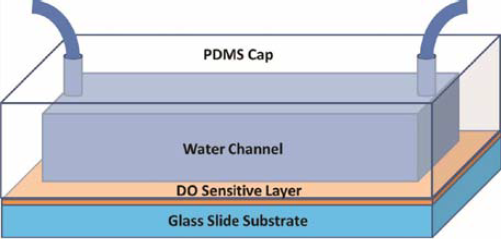
\includegraphics[width=3in]{jsenga.png}%
%\end{wrapfigure}%
\begin{abstract}
Magnetic 3D motion tracking that externally excites small, lightweight, wireless, battery-less inductor-capacitor (LC) coils according to the principle of electromagnetic induction and tracks each LC coil using an externally located flux sensor array, is supposed to cover the area where optical or inertial systems cannot handle well due to its characteristics. However, there is the principle’s inherent dead-angle problem that makes tracking impossible in certain configurations of the LC coil, making stable tracking difficult. To solve this problem, we propose a practical 3D motion tracking system that uses a novel multi-axis marker consisting of multiple LC coils with the same resonance frequency to achieve reliable tracking. Since the complex electromagnetic relationships of the proposed markers make it extremely difficult to calculate the results with a classical numerical model, we solve by using deep learning to learn the regression from the simulation flux values to the 3D configuration of the markers. The proposed markers can be tracked stably in any configuration and with the same level of accuracy as a single LC coil, solving the dead angle problem. The proposed small, lightweight, wireless markers do not require power supply, and can robustly track very long movements. Our method is suitable for tasks that are difficult to track with existing motion tracking systems. We also built some examples to show how well our system works for actual situations.

\end{abstract}

\begin{IEEEkeywords}
3D user interface, deep learning, magnetic sensors, motion capture, virtual reality.
\end{IEEEkeywords}
\end{minipage}}}

\maketitle

\section{Introduction}
\label{sec:introduction}
\IEEEPARstart{M}{otion} tracking technology plays an important role in various fields such as virtual reality, computer animation, and robotics, and its demand is high. However, dexterous 3D motion tracking requires tracking of multiple targets that are small and easily occluded. For example, movements of fingers and objects operated by fingers can be considered. To accomplish these tasks, the markers used in a motion tracking system need to be small, lightweight, identifiable, wireless, and occlusion-free, which remains difficult.

The magnetic systems are widely used because they are highly accurate and occlusion-free. Methods of tracking the movement of permanent magnets using magnetic sensors has been proposed \cite{gaussbits, gaussrfid, utrack}, however since the signal strength is weak, this method can only be realized by tracking at a short distance. Methods has been proposed in which markers that combine a permanent magnet and an inertial sensor is used, and the configurations of the markers is calculated from the magnetic field of the permanent magnet measured by a magnetometer and the data measured by the inertial sensor \cite{fem, magne_inert}. Several methods using electromagnets have also been proposed \cite{polhemus, intr_cap_magne_sens, finexus}, however these methods can accurately track markers over a wider range, however require wired power supply or sensor data transmission, which interferes with dexterous motion tracking tasks. A self-contained system that does not require a wired power supply due to wearable hardware with a battery has been proposed, however the drive time is limited, and a larger battery causes a failure in the tracking task \cite{auraring}.
A tracking method using an induction coil has also been proposed to solve the power supply limitation \cite {paperio}. Based on this technique, a magnetic 3D motion tracking system \cite{im3d, im6d, yabukami1, hashi1} with small, lightweight, identifiable, wireless, and occlusion-free markers is useful for dexterous motion tracking tasks. This system uses a passively induced small and lightweight inductor-capacitor (LC) coil as a marker and embeds flux sensors in the measurement space to enable tracking of the movement of small objects. However, this system has the dead-angle problem in principle. Since the excitation signal generated by the exciting coil for exciting the LC coil has a specific direction, the LC coil is not excited when the LC coil is perpendicular to the exciting signal, and tracking fails. We define this configuration as the dead-angle. To solve this problem, a multi-axis marker consisting of three LC coils with different resonance frequencies has been proposed \cite{im6d}. However, due to the limited frequency generation range of the hardware, the maximum number of markers that can be used simultaneously in the system is reduced to 1/3. Structure-aware temporal bilateral filter (SATBF) for reconstructing a motion sequence with the dead-angle has been proposed \cite{im3d+}. However, in the case of a long-term dead-angle that exceeds the time window size of the filter, the motion sequence cannot be reconstructed correctly, and the time window size affects the real-time delay.

In this work, we propose a multi-axis marker consisting of multiple LC coils with the same resonance frequency in order to solve a long-term dead angle without reducing the number of markers that can be used simultaneously. By configuring the markers with LC coils that all have the same resonance frequency, the number of markers that can be used simultaneously is not reduced without occupying the frequency range of the hardware. In addition, the dead angle problem that occurs in the case of a conventional single LC coil can be solved by using a multi-axis marker. However, due to the complicated electromagnetic relationship between each LC coil in the same marker, the numerical solution approach proposed by \cite {im6d} is difficult. Therefore, we propose a new deep learning (DNN) computational framework. DNN allows the analysis of complex physical models, and marker tracking much faster than numerical solutions.

\section{Related Work}


\section{Magnetic 3D motion tracking system}
\label{overview}
In this section, we describe the tracking principle of our system that uses small, lightweight, identifiable, and passive markers. Next, we describe the principle’s inherent dead-angle problem.

\subsection{Tracking principle}
The overview of our system is shown in Fig. \ref{overview_im3d}, and the hardware setup is shown in Fig. \ref{hardware_setup}.
\begin{figure}[!t]
    \centerline{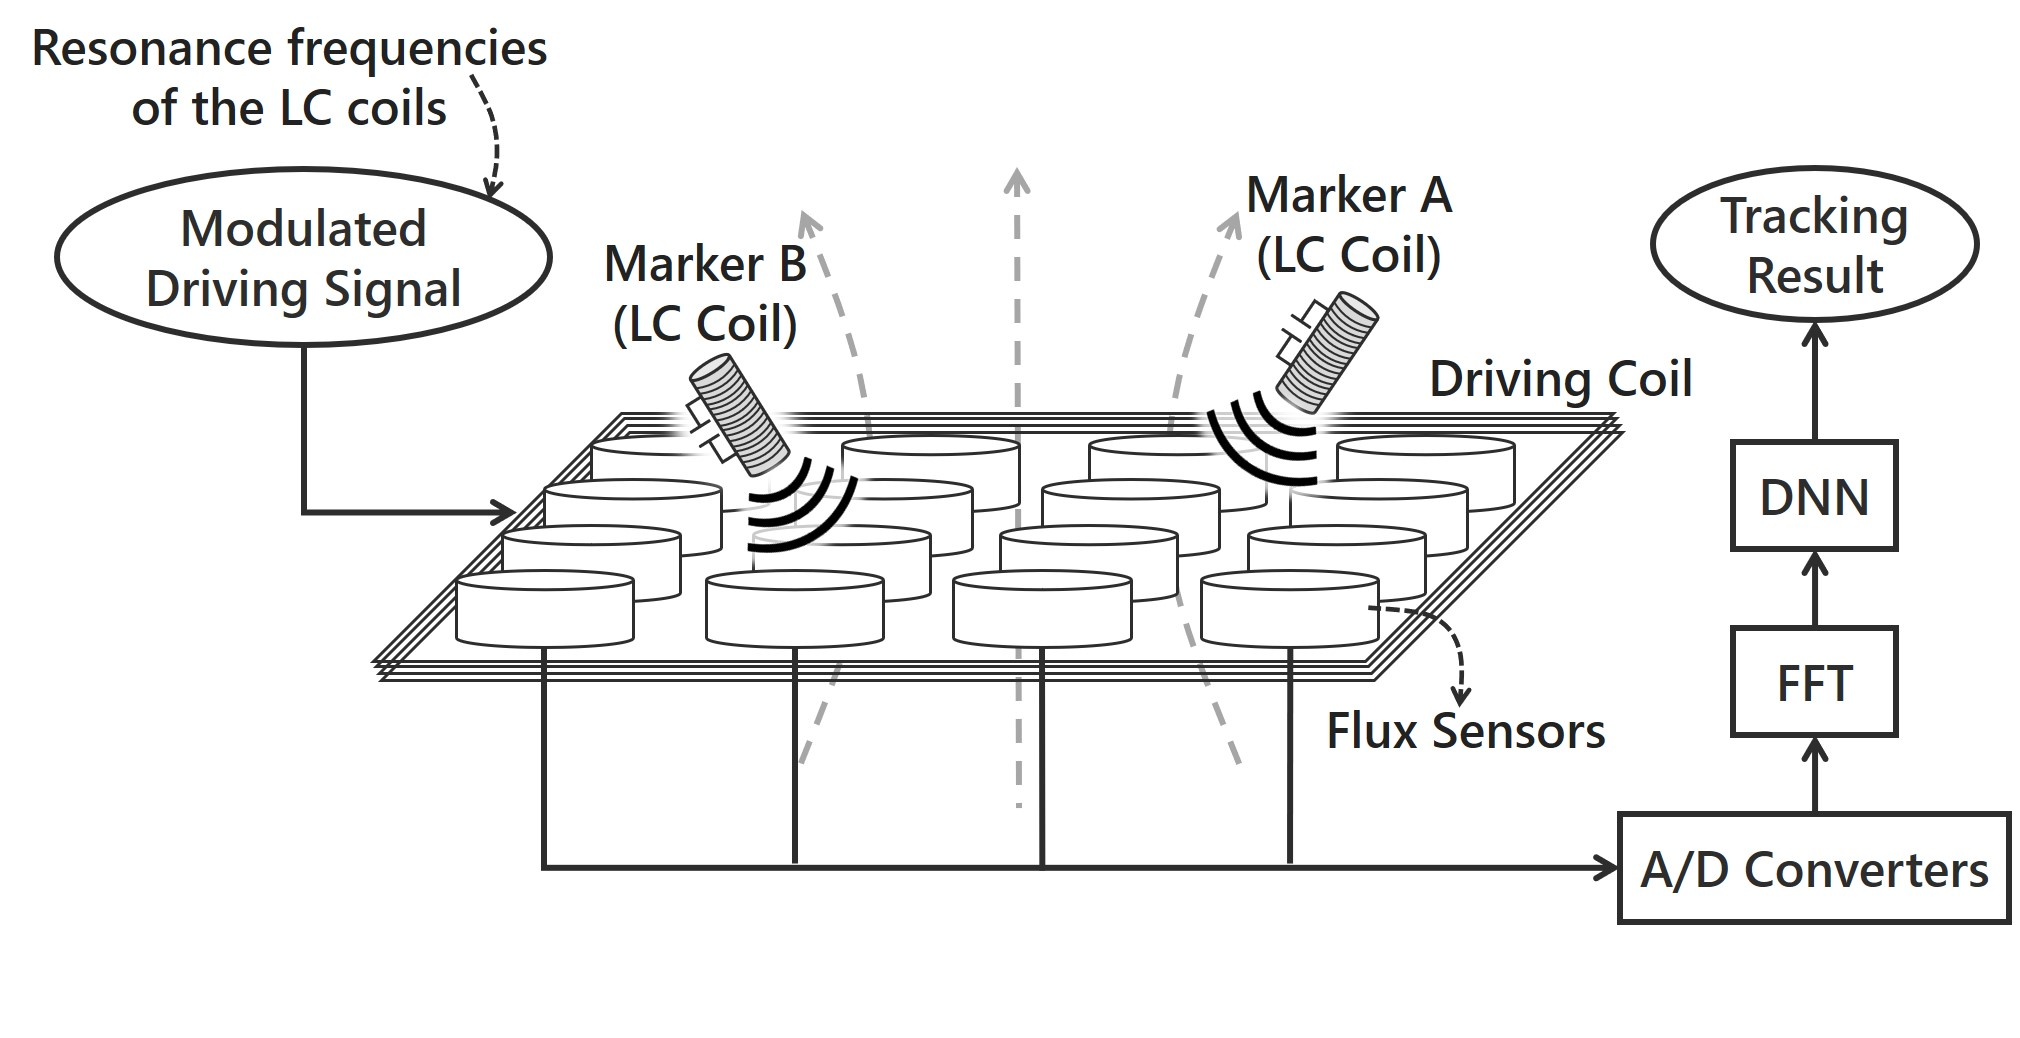
\includegraphics[width=\columnwidth]{figure/overview_proposed.jpg}}
    \caption{System overview}
    \label{overview_im3d}
\end{figure}
\begin{figure}[!t]
    \centerline{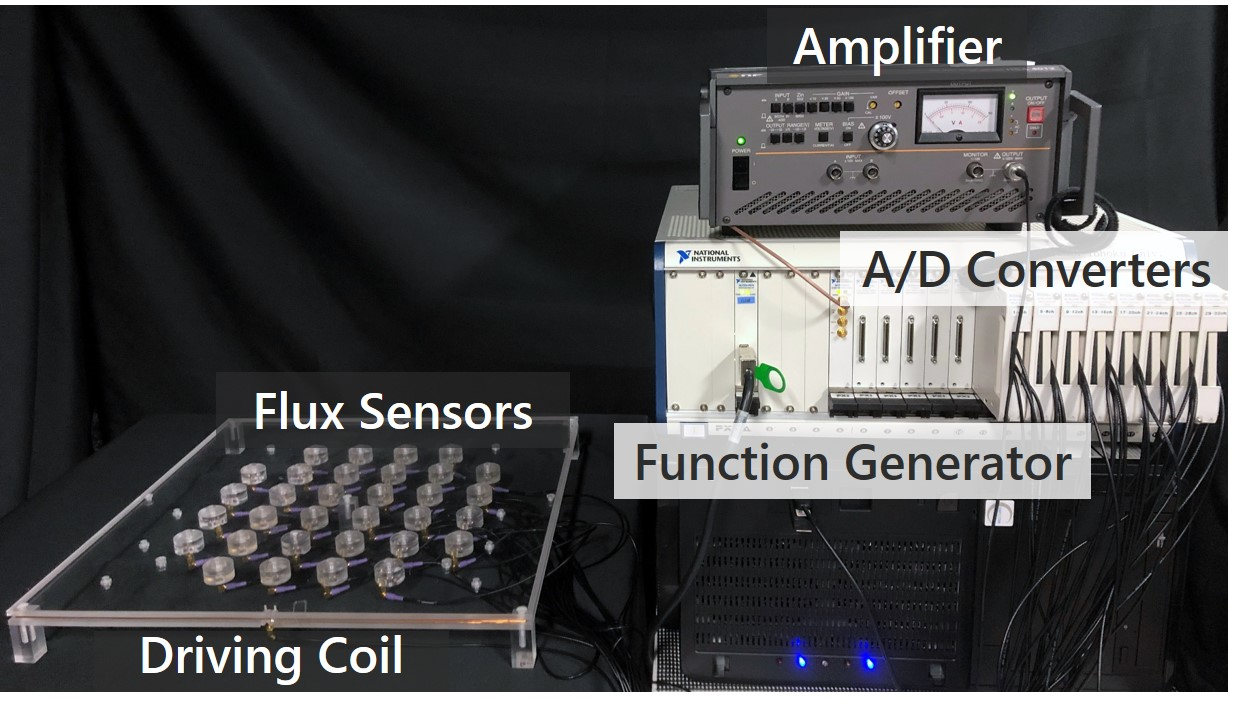
\includegraphics[width=\columnwidth]{figure/hardware_setup.jpg}}
    \caption{Hardware setup}
    \label{hardware_setup}
\end{figure}
\begin{figure}[!t]
    \centerline{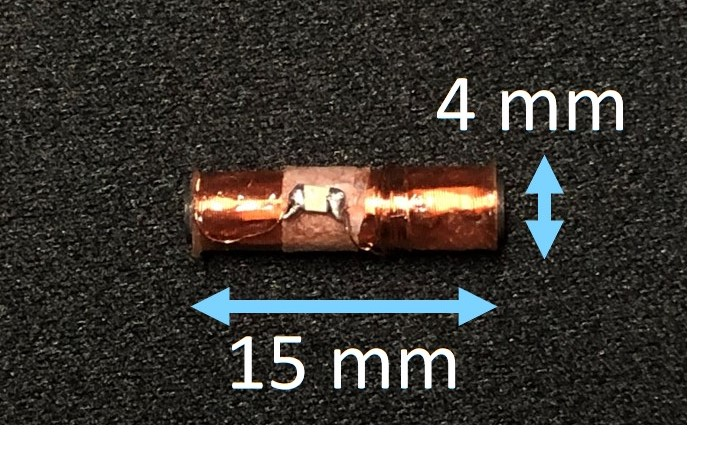
\includegraphics[width=50mm]{figure/LCcoil2.jpg}}
    \centering
    \caption{LC coil}
    \label{lc_coil}
\end{figure}


As shown in Fig. \ref{overview_im3d}, an exciting magnetic field is generated by the modulation current generated by the function generator flowing through the exciting coil. When a small and lightweight LC coil (Fig. \ref{lc_coil}) used as a marker in the system is inserted in the exciting magnetic field, the LC coil is excited and a resonance magnetic flux is generated. Next, the resonant magnetic field is measured as an induced voltage by flux sensors placed in the measurement space, converted by an A/D converter, and then used by a computer to calculate the position and orientation of the LC coil. In addition, each LC coil has different resonance frequency characteristics, and by applying a signal including the resonance frequency of the LC coils used for tracking to the exciting coil, multiple LC coils can be excited at the same time. The output of each LC coil can be obtained by FFT analysis of the induced voltage measured by the flux sensors.

Next, we describe the relationship between the spatial arrangement of the LC coil and the induced voltage of the flux sensors. Assuming that the magnetic flux density generated by the marker can be regarded as a magnetic dipole field, according to Biot-Savart's law, the induced voltage of the magnetic flux sensor located at the origin by the LC coil of configuration ${\bf C}=({\bf r}, \theta, \phi)$ can be computed as
\begin{equation}
  B({\bf C}) =  \frac{\mu_{0}}{4\pi} \left\{
  -\frac{{\bf M}}{\|{\bf r}\|^{3}}
  +\frac{3({\bf M} \cdot {\bf r}){\bf r}}{\|{\bf r}\|^{5}}
  \right\}\cdot \bf v
  \label{biot-savert}
\end{equation}

where $B$ is the magnetic flux density, and ${\bf M}$ is the magnetic moment with the direction of the LC coil represented by $\theta$ and $\phi$ and the magnitude represented by scalar ${M}$. ${\bf r}$ is the 3D position of the LC coil, and ${\bf v}$ is the unit vector representing the direction of the flux sensor. After the above process, the 3D position, orientation, and magnetic moment of the LC coil can be obtained.

Using (\ref{biot-savert}) and the induced voltage at each flux sensor, the configuration ${\bf C}$ of each LC coil can be computed. In a previous work \cite{im3d, im6d, yabukami1, hashi1}, ${\bf C}$ was numerically solved by the Gauss-Newton method, however the complex electromagnetic relationships of the proposed marker described in section \ref{proposed marker} make it extremely difficult to calculate the results with the classical numerical model. In this work, we successfully solve this problem with DNN method described in section \ref{dnn}.

\subsection{Dead-angle problem}
Since the direction of the magnetic field generated by the exciting coil is constant, if the LC coil is perpendicular to the direction of the magnetic field generated by the exciting coil, the LC coil is not excited and the correct tracking result cannot be calculated. We define this configuration of the LC coil as the dead-angle. The tracking principle based on electromagnetic induction essentially causes the dead-angle problem.

In order to solve the dead-angle problem, various approaches have been examined so far. In \cite{im6d}, by arranging three LC coils with different resonance frequencies in different configurations in the same marker, at least one LC coil can always be used without dead-angle in any configurations of the marker. However, since this method uses LC coils with three different resonance frequencies for the markers, there is a problem that the number of markers that can be used simultaneously on the system is reduced to 1/3. \cite{im3d+} proposes a method of reconstructing a motion sequence with the dead-angle and unstable tracking results using SATBF. SATBF is a method of smoothing a motion sequence whose tracking has become unstable due to the dead-angle and reconstructing a smooth marker motion. However, if a long-term dead-angle occurs that exceeds the filter time window, the motion cannot be reconstructed correctly.
Also, a method to solve the dead-angle using multiple exciting coils has been proposed \cite{four_ext_coil}. In this method, it was shown that by exciting the LC coil with four exciting coils arranged at different positions, the LC coil can be tracked stably regardless of the configuration, however the strength of the resonance magnetic field generated by the LC coil is weaker than when a single exciting coil is used, which affects the decrease in accuracy and the limitation of the measurement space.

In this work, we propose a method that can solve long-term dead-angle without reducing the number of markers that can be used simultaneously on the system by arranging multiple LC coils with the same resonance frequency in different configurations to compose a marker.

\section{3D position calculation of markers}
\label{dnn}
The proposed marker is difficult to calculate with the numerical model by the Gauss-Newton method proposed in \cite{im3d, im6d, yabukami1, hashi1} due to its complicated electromagnetic relationship. Therefore, we use DNN to predict the 3D position of the marker. In this section, we first describe the data collection by an extension of the theoretical formula explained in Section \ref{overview}, and then describe the structure and learning process of our neural network.
\subsection{Training data}
In order to efficiently collect a large amount of training data, we used simulation data that theoretically calculated the resonance magnetic flux of the marker measured by the flux sensors using a theoretical formula. When the marker is composed of multiple LC coils with the same resonance frequency, assuming that the induced voltage measured by the magnetic flux sensor is not affected by cross-coupling  \cite {cross-coupling, cross-coupling2} due to the interference of magnetic flux between LC coils in the same marker and the induced strength of each LC coil is equal, the induced voltage of each LC coil is totaled. The induced voltage of the flux sensor located at the origin by each LC coil of the marker at the 3D position and orientation ${\bf C}_{i}=({\bf r}_{i}, \theta_{i}, \phi_{i}) $($i:$ LC coil number in the same marker) is calculated by (\ref{biot-savart-extension}).

\begin{IEEEeqnarray}{rCl}
 {\sum_{i} B({\bf C}_{i})} \hspace{180px}\nonumber\\
  = \sum_{i} \frac{\mu_{0}}{4\pi} \left\{
  -\frac{{\bf M}_{i}}{\|{\bf r}_{i}\|^{3}}
  +\frac{3({\bf M}_{i} \cdot {\bf r}_{i}){\bf r}_{i}}{\|{\bf r}_{i}\|^{5}}
  \right\}\cos\psi_{i}\cdot \bf v
  \label{biot-savart-extension}
\end{IEEEeqnarray}

where $i$ is the LC coil number in the same marker, ${\bf M}_{i}$ is the magnetic moment of each LC coil, ${\bf v}$ is the unit vector in the direction of the flux sensor, and ${\bf r}_{i}$ is the 3D position of each LC coil, ${\psi_{i}}$ is the angle between the magnetic flux vectors generated by the exciting coil which is calculated by simulation and the direction vector of each LC coil ${\bf M}_{i}$\cite{squarecoil}. Equation (\ref{biot-savart-extension}) allows the induced voltage $\bf B$ $= (B_{1},\dots ,B_{N})$ measured by the flux sensors to be calculated from the resonant magnetic flux of the marker at the 3D position ${\bf r}$. Here, $N$ is the flux sensor number. This makes it possible to collect a large number of $(\bf B,\bf r)$ pairs in the measurement space.

\subsection{Network structure}
We used a feedforward neural network to regress measurements at the flux sensors to the 3D positions of the markers. Our network is composed of several fully connected layers, each of which is followed by RELU activation functions:
\begin{IEEEeqnarray}{rCl}
   {\Phi ({\bf X}; {\boldsymbol \beta})} = {\bf W_{4}} {\rm RELU} ({\bf W_{3}} {\rm RELU} ({\bf W_{2}} \hspace{60px}\nonumber \\
   {\rm RELU} ({\bf W_{1}} {\rm RELU} ({\bf W_{0}} {\bf X} + {\bf b_{0}}) + {\bf b_{ 1}}) + {\bf b_{3}}) + {\bf b_{4}})
\end{IEEEeqnarray}
where ${\bf X}$ is the input vector, ${\boldsymbol \beta} = ({\bf W_{0}}, {\bf b_{0}}, \dots, {\bf W_{4} }, {\bf b_{4}}) $ are the network weights and biases. Here we used four fully connected layers with hidden unit numbers of 1024, 2048, 4096, and 1024.

\subsection{Training}
To train the network, we minimized the following loss function based on the mean square error (MSE) using a stochastic gradient descent:
\begin{equation}
Loss=\|\Phi({\bf X};{\boldsymbol\beta}) - C\|^{2} + \gamma|{\boldsymbol\beta}|
\end{equation}
where C is the ground-truth configuration of the marker and the second term is the L2 regularization term. In our study, $\gamma$ was set to 0.0001.

The system was implemented in Keras \cite{keras} with Tensorflow \cite{tensorflow}, and we used an Adam solver \cite{adam} to speed up the convergence. Training was performed for each of the marker with three LC coil and four LC coil until the loss reached less than 0.02.

\section{Multi-axis Marker}
\label{proposed marker}
\subsection{Resonance frequency characteristics of LC coils}
In this work, the proposed marker design consists of multiple LC coils with different axes, and to solve the problem of reducing the number of markers that can be used simultaneously, each LC coil that composes a marker has been tuned to have the same resonant frequency characteristics. However, since the LC coil set used for a marker was manufactured by hand, there are individual differences in the resonance frequency characteristics of each LC coil\ref{freq-charac-diff}. When actually using the LC coil set as a marker, perform FFT analysis by selecting one frequency with almost the same induced strength of each LC coil.

\subsection{LC coil placement requirements within the same marker}
When multiple LC coils with similar resonance frequencies are placed at close range, cross-coupling occurs in which the resonance frequency characteristics shift due to the interference of the magnetic fluxes of each other \cite {cross-coupling, cross-coupling2}. Since the frequency shift due to cross-coupling changes dynamically depending on the angle of each LC coil, a marker design that reduces the influence of cross-coupling is required in order to apply our DNN model.

In order to design the optimum marker, we designed three prototypes, a marker with the same design as that proposed in the previous work \cite {im6d}, a compact marker in which each LC coil was placed orthogonally and closely attached, and each LC coil was placed orthogonally at a distance of 1 [cm] or more. We rotated each prototype from 0$^\circ$ to 90$^\circ$ at intervals of 30$^\circ$ with the X axis as the rotation axis, and verified the effect of cross-coupling by comparing the measured value of the magnetic flux sensor with the theoretical value calculated by (\ref{biot-savart-extension}).
The results are shown in Fig. \ref{freq_charac}.

As a result, it was confirmed that the frequency peak of prototype (a) deviates from the original resonance frequency characteristics of each LC coil, and the resonance frequency characteristics change depending on the attitude of the marker. This is considered because the relative angle of each LC coil is 60$^\circ$, and cross-coupling occurs due to the influence of the magnetic flux vector components of each LC coil.
Similarly, it was confirmed that the resonance frequency characteristics of the marker change depending on the attitude of Prototype (b). This suggests that the distance between LC coils is also an important factor in cross-coupling.
It was confirmed that in Prototype (c), the peak of the resonance frequency of the marker did not change significantly even if the marker configuration was changed. Therefore, it was shown that the optimum marker design condition is to arrange the LC coils orthogonally to each other and keep the distance by 1 [cm] or more.

\begin{figure}[t]
    \centerline{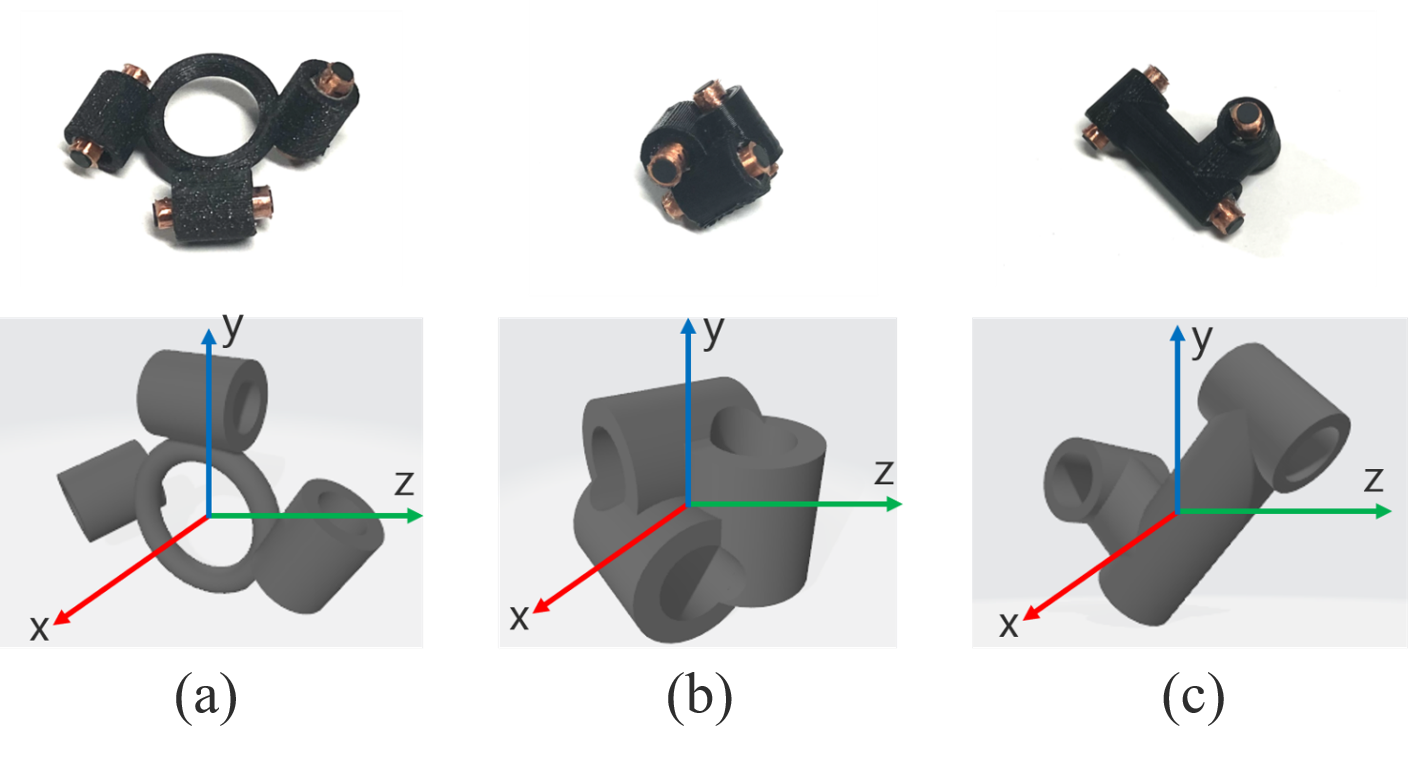
\includegraphics[width=\columnwidth]{figure/marker_prototype2.png}}
    \caption{Prototype marker. (a) The relative angle of each LC coil is 60$^\circ$ and  placed on the ring. (b) The relative angle of each LC coil is 90$^\circ$ and placed in close each other. (c) The relative angle of each LC coil is 90$^\circ$ and placed at least 1 [cm] apart.}
    \label{marker_prototype}
\end{figure}

\begin{figure*}[t]
\centerline{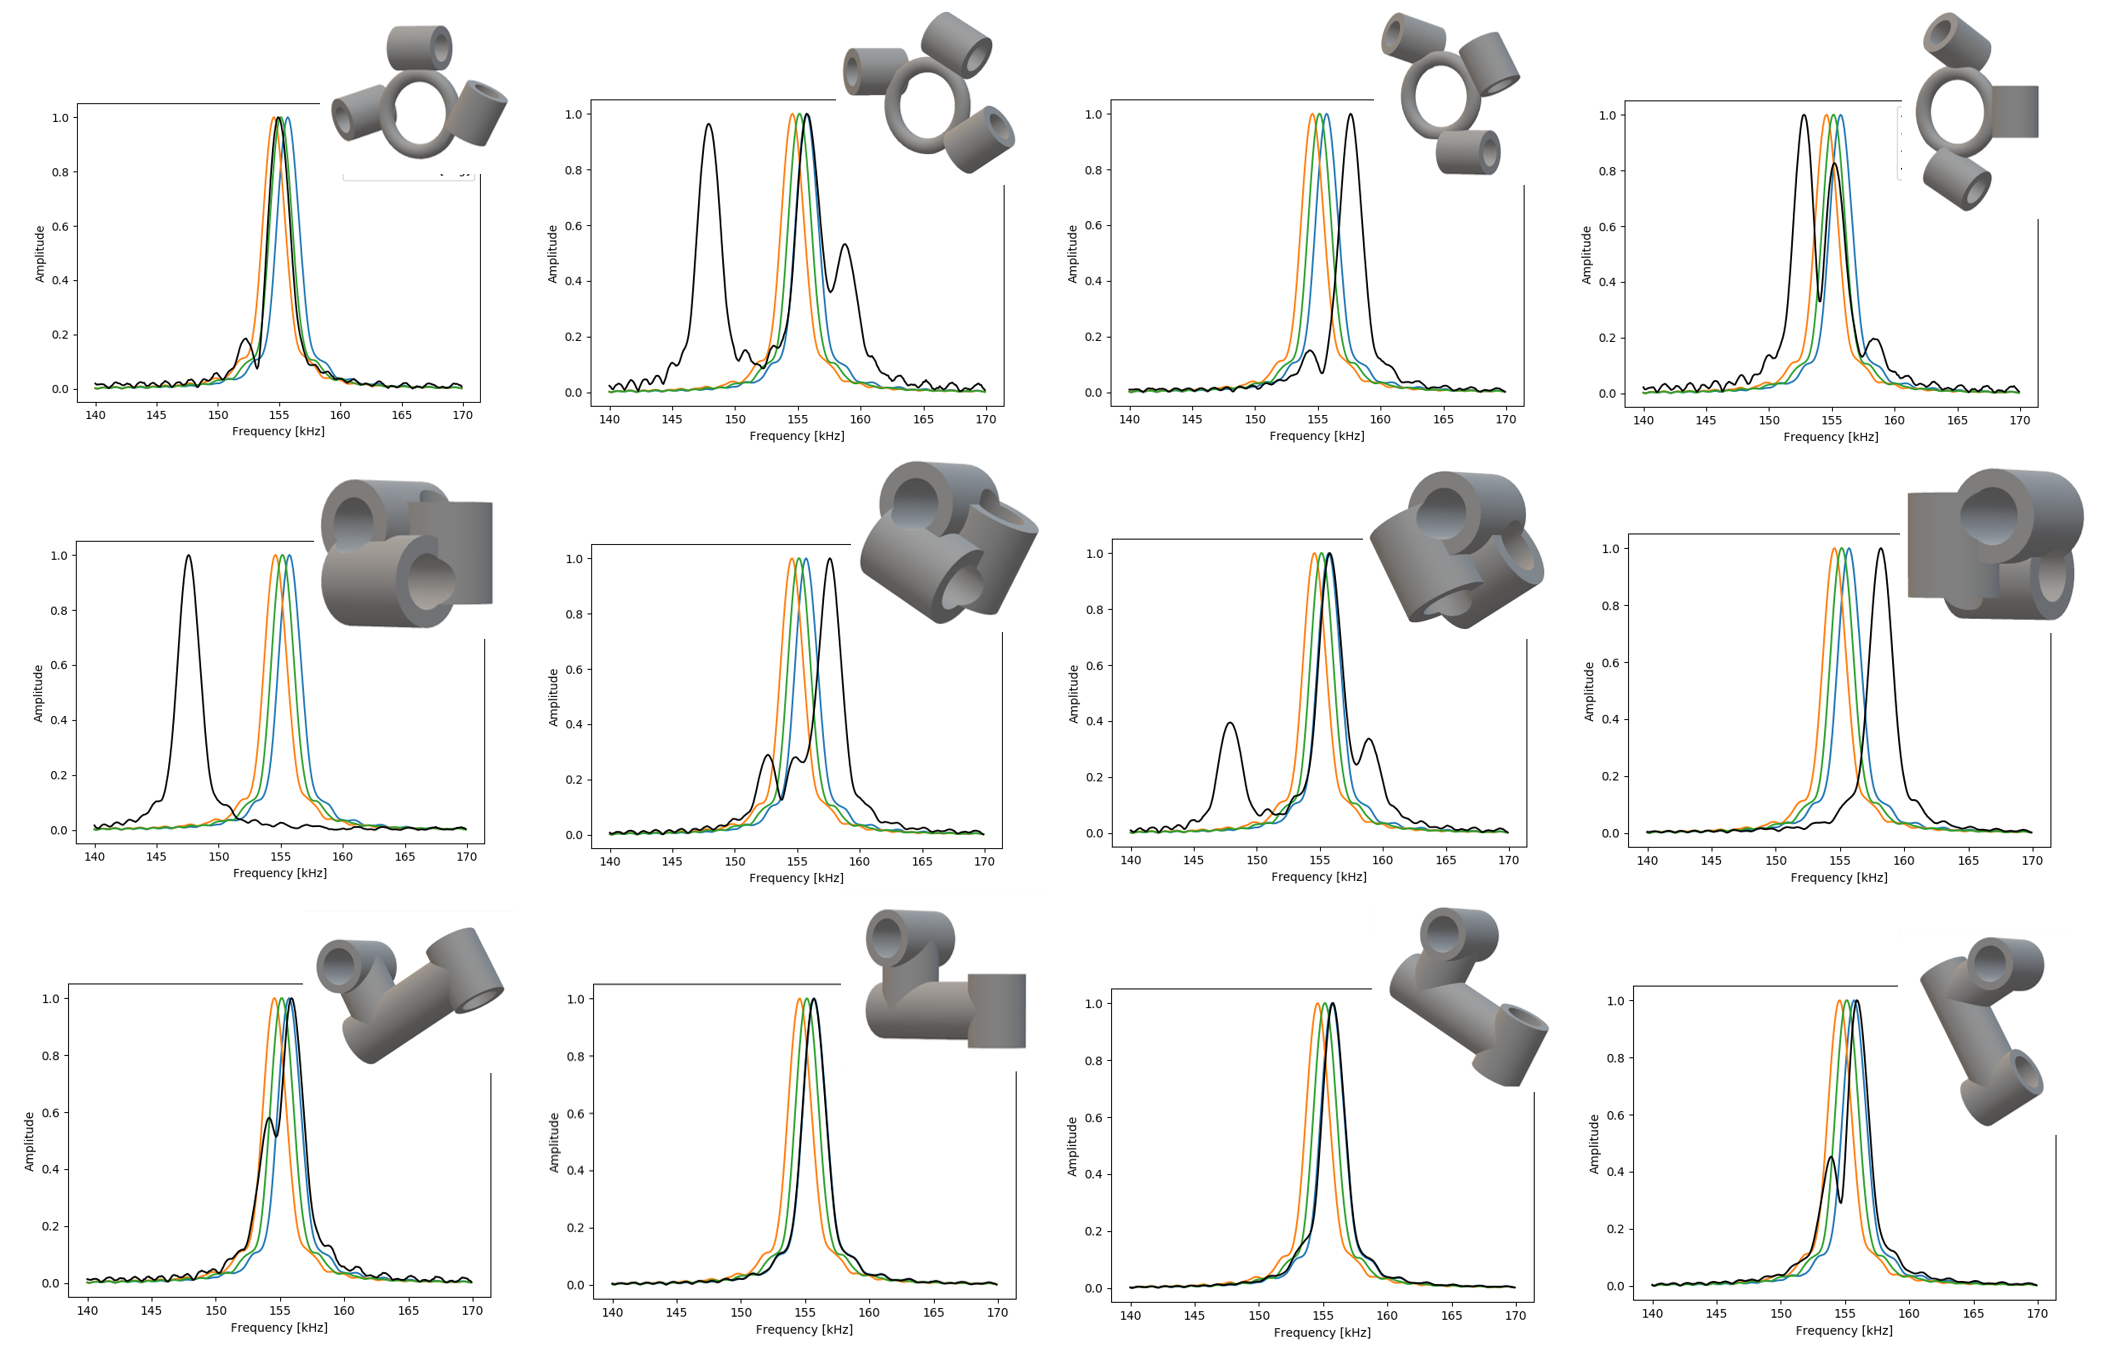
\includegraphics[width=2\columnwidth]{figure/frequency_characteristics.png}}
    \caption{Resonance frequency characteristics of Prototype markers: Resonance frequency of each LC coil in the same marker (blue, orange, green), Resonance frequency of the marker (black).}
    \label{freq_charac}
\end{figure*}

\subsection{Marker design}
We created two types of marker that satisfy the design requirements of prototype (c). 

First, we made a marker with the same design as the prototype (c), in which three LC coils were orthogonal to each other and placed at a distance of 1 [cm] or more from each other. The weight is $<$ 4.0 [g] (depending on the number of turns of the LC coil), and the dimensions are as shown in the Fig. \ref{marker_size} (a). 

Next, as with the marker containing three LC coils, we made a marker in which the four LC coils were orthogonal to each other and placed at a distance of 1 [cm] or more from each other. The weight is $<$ 5.5 [g] (depending on the number of turns of the LC coil), and the size is as shown in the Fig. \ref{marker_size} (b). 

By arranging multiple LC coils in different configurations, one of the LC coils can always be used, therefore the dead-angle can be solved, and even if the configuration of the marker changes, the frequency characteristics do not change significantly, and the contribution of the marker's induced voltage can be calculated correctly by FFT analysis.

\begin{figure}[!t]
    \centerline{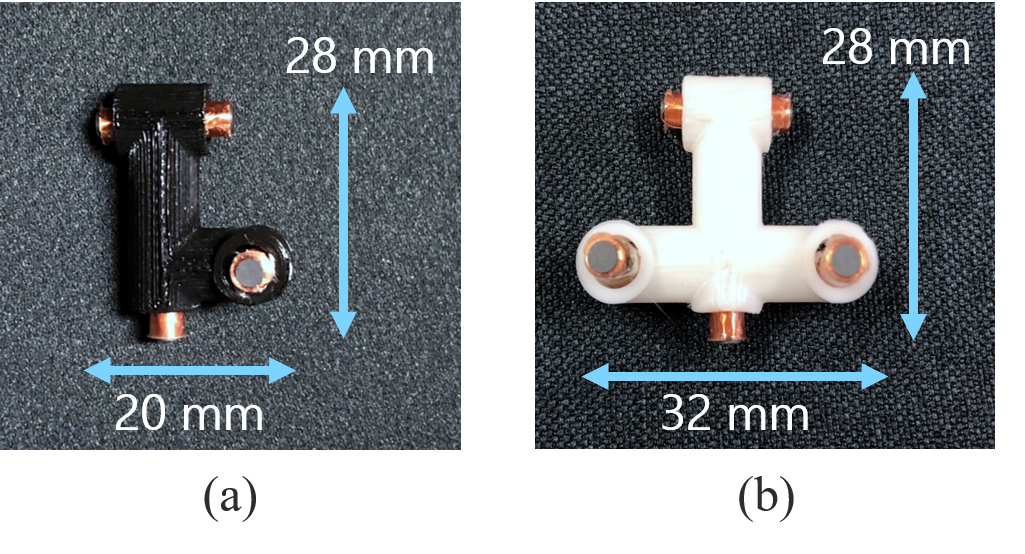
\includegraphics[width=\columnwidth]{figure/marker_size.png}}
    \caption{Proposed marker with (a) three LC coils, (b) four LC coils.}
    \label{marker_size}
\end{figure}

\section{Evaluation}
\subsection{Stability}
In order to evaluate the validity of the marker design proposed for solving the dead-angle problem, we conducted an experiment to rotate the marker 360 $^\circ$ on a plane with the flux sensor array. We compared the mean values of the outputs of the 32 magnetic flux sensors when the markers were rotated with a single LC coil and two proposed markers. Using a coordinate system in which the XZ plane is horizontal to the flux sensor array and the XY plane is perpendicular to the origin of the center of the flux sensor array. As shown in Fig. \ref{rotation-define}, each marker was rotated 360 $^\circ$ with the X and Z axes as the rotation axes. The output of the flux sensor and rotation angle of a single LC coil and proposed marker with three LC coils are shown in Fig. \ref{angle_characteristics_3LC}. A single LC coil and proposed marker with four LC coils are shown in Fig. \ref{angle_characteristics_4LC}.

In the case of a single LC coil, it can be seen that the output of the flux sensors becomes very weak around the configuration perpendicular to the direction of the exciting magnetic flux (90$^\circ$, 270$^\circ$). In this configuration, the DNN cannot accurately estimate the 3D position of the LC coil, resulting in the dead-angle. On the other hand, the outputs of the two types of proposed markers stably maintain a constant strength at any rotation angles. Therefore, the proposed markers show that tracking can be continued stably in any configuration and that the dead-angle problem that occurs with a single LC coil can be solved.

\begin{figure}[!t]
    \centerline{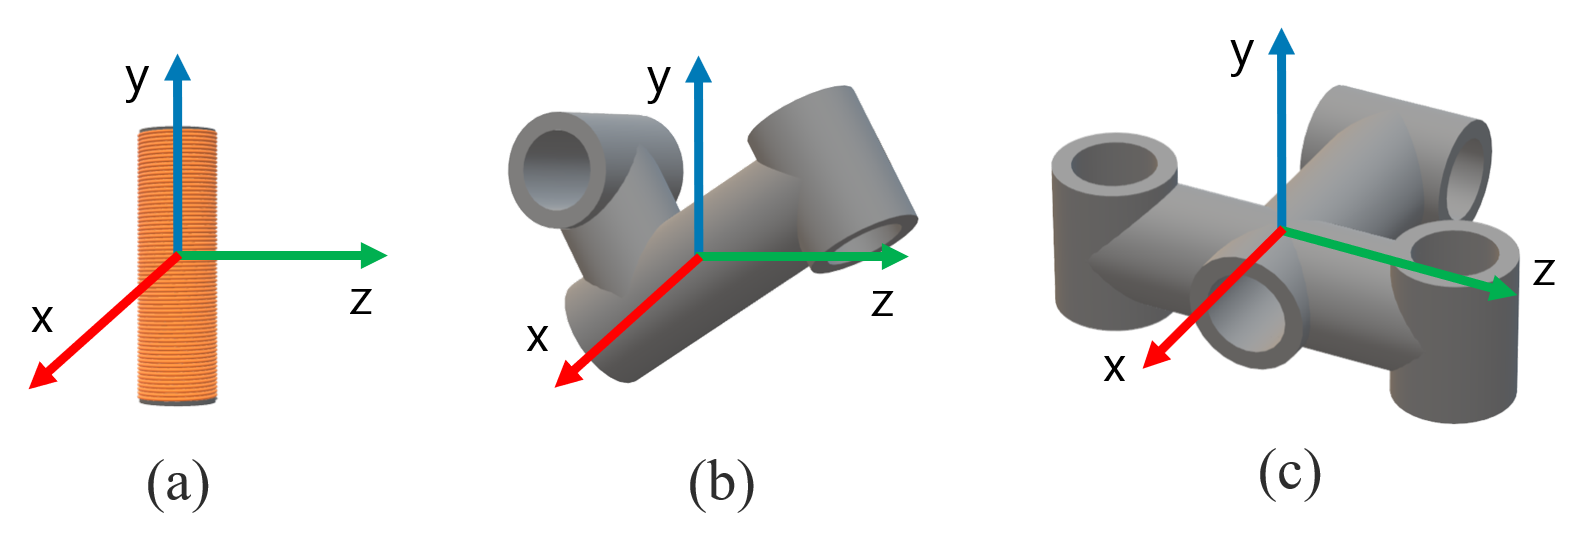
\includegraphics[width=\columnwidth]{figure/rotation-define3.png}}
    \caption{Rotation axis. (a) Single LC coil. (b) Proposed marker with 3 LC coils. (c) Proposed marker with 4 LC coils.}
    \label{rotation-define}
\end{figure}

\begin{figure}[!t]
    \centerline{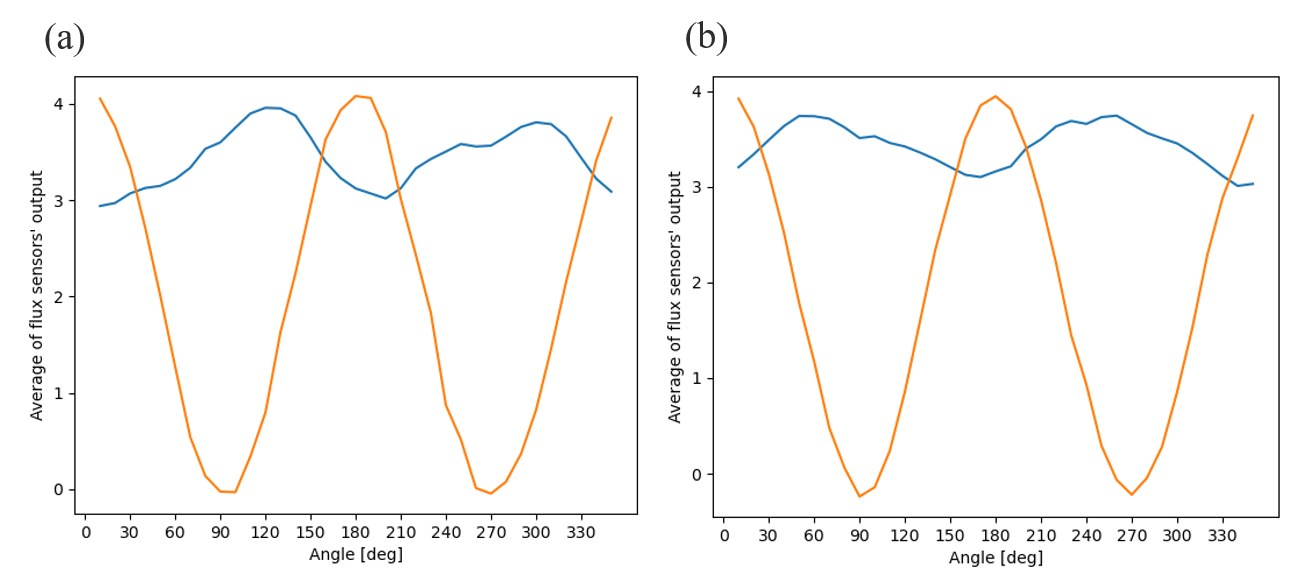
\includegraphics[width=\columnwidth]{figure/angle_characteristics_3LC.png}}
    \caption{Average of flux sensors' output of single LC coil and proposed marker with 3 LC coils. (a) X axis rotation. (b) Z axis rotation.}
    \label{angle_characteristics_3LC}
\end{figure}
\begin{figure}[!t]
    \centerline{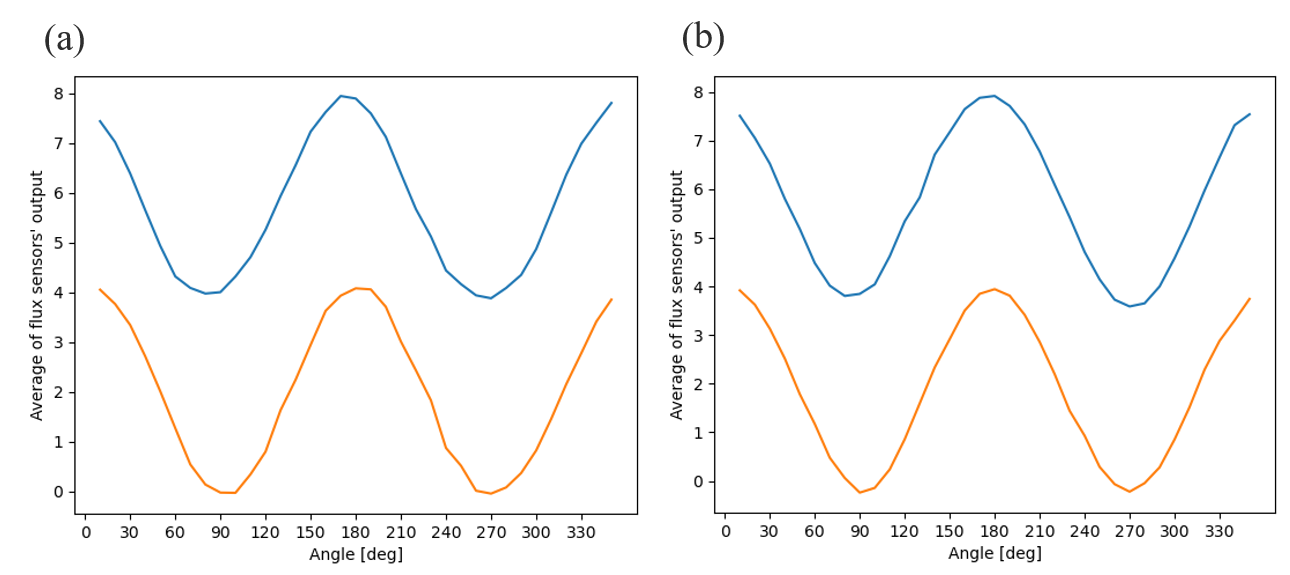
\includegraphics[width=\columnwidth]{figure/angle_characteristics_4LC.png}}
    \caption{Average of flux sensors' output of single LC coil and proposed marker with 4 LC coils. (a) X axis rotation. (b) Z axis rotation.}
    \label{angle_characteristics_4LC}
\end{figure}

\subsection{Accuracy}
Accuracy is an important factor in motion tracking systems. We compared the accuracy of the position calculation of two types of proposed markers and a single LC coil with some simple motions with the marker orientation constant. The markers ware attached to the tip of the robot arm (Nachi MZ701 with positional error less than 1 [mm]) for measurement, and the ground truth was the coordinates of the tip of the robot arm.

In order to measure the error in the vertical direction, the XZ plane is defined to be horizontal to the flux sensor array, and we moved the markers from 0.044 [m] to 0.15 [m] in height along the Y axis at some coordinates on the XZ plane. The coordinates on the XZ plane are in the range of 1/8 on the XZ plane due to the symmetry of the flux sensor array.

We compared the tracking accuracy of a single LC coil and two types of proposed markers. The orientation of each marker was set to intervals of 30$^\circ$ from 0$^\circ$ to 90$^\circ$ with the X axis and Z axis as the rotation axes, respectively. When rotated 90$^\circ$ with the X-axis or Z-axis as the rotation axis, a single LC coil becomes a dead angle. The tracking results is shown in Fig. \ref{y-axis-tracking}. The mean absolute error (MAE) of tracking is shown in Fig. \ref{y-axis-ave_error}. The error bar shows the standard deviation. In addition, Table \ref{y-axis-error_1LC}, Table \ref{y-axis-error_3LC} and Table \ref{y-axis-error_4LC} are show the MAE, maximum and minimum errors of the tracking of a single LC coil and the proposed marker.

\begin{figure*}[t]
  \begin{minipage}{0.5\hsize}
  \begin{center}
   \centerline{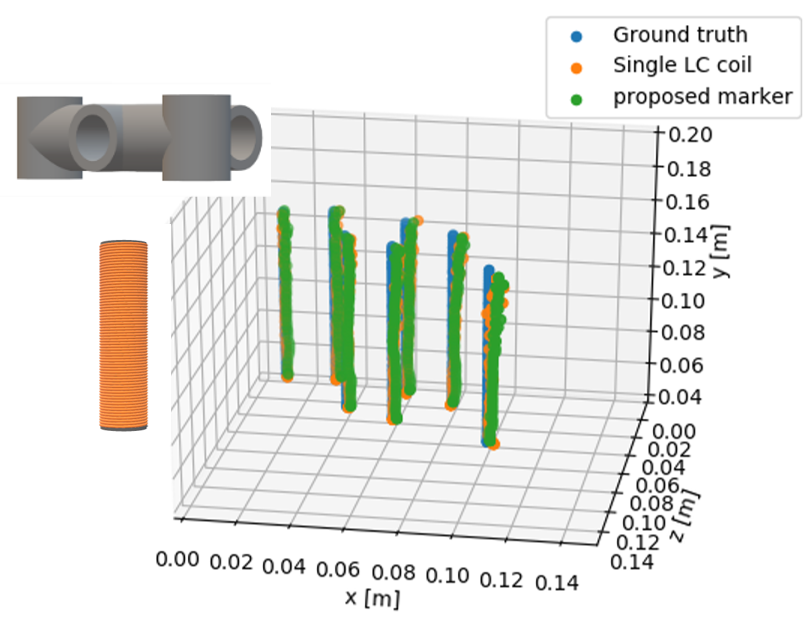
\includegraphics[width=65mm]{figure/yaxis_x-axis_0deg_4LC_2.png}}
  \end{center}
 \end{minipage}
  \begin{minipage}{0.5\hsize}
  \begin{center}
   \centerline{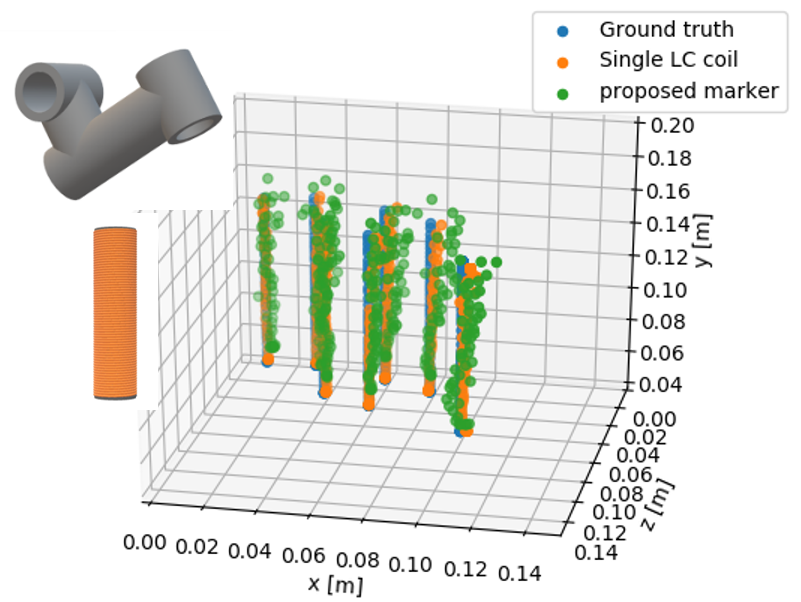
\includegraphics[width=65mm]{figure/yaxis-x0_2.png}}
  \end{center}
 \end{minipage}
 \begin{minipage}{0.5\hsize}
  \begin{center}
   \centerline{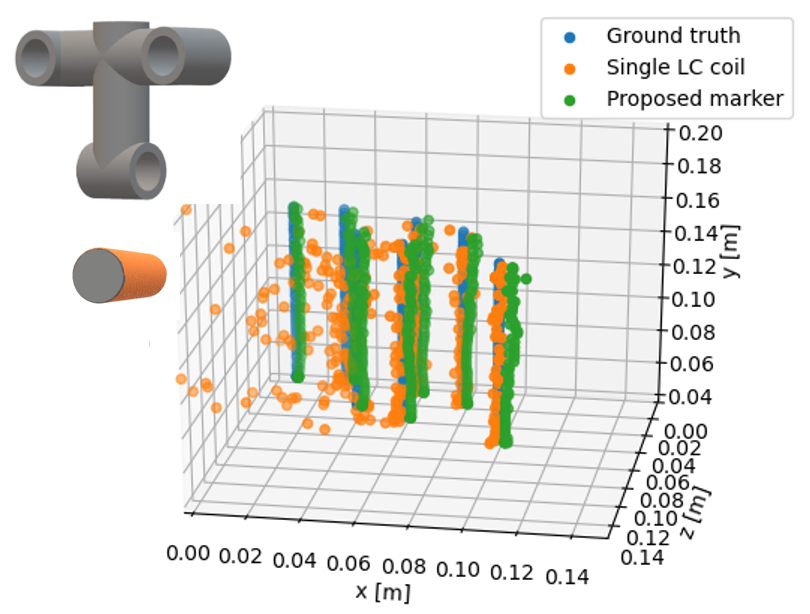
\includegraphics[width=65mm]{figure/yaxis_z-axis_90deg_4LC_2.png}}
  \end{center}
 \end{minipage}
 \begin{minipage}{0.5\hsize}
  \begin{center}
   \centerline{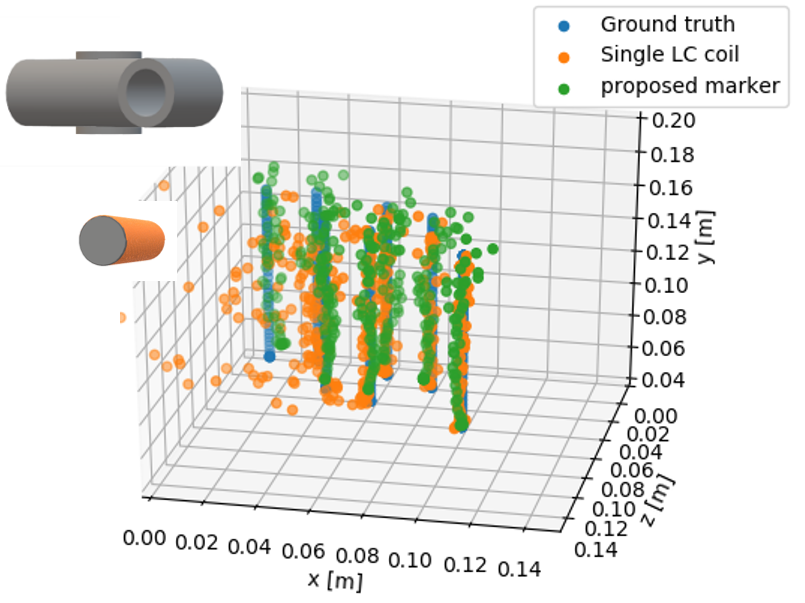
\includegraphics[width=65mm]{figure/yaxis-z90_2.png}}
  \end{center}
 \end{minipage}
 \caption{Y-axis motion tracking results}
 \label{y-axis-tracking}
\end{figure*}
 
 \begin{figure}[t]
    \centerline{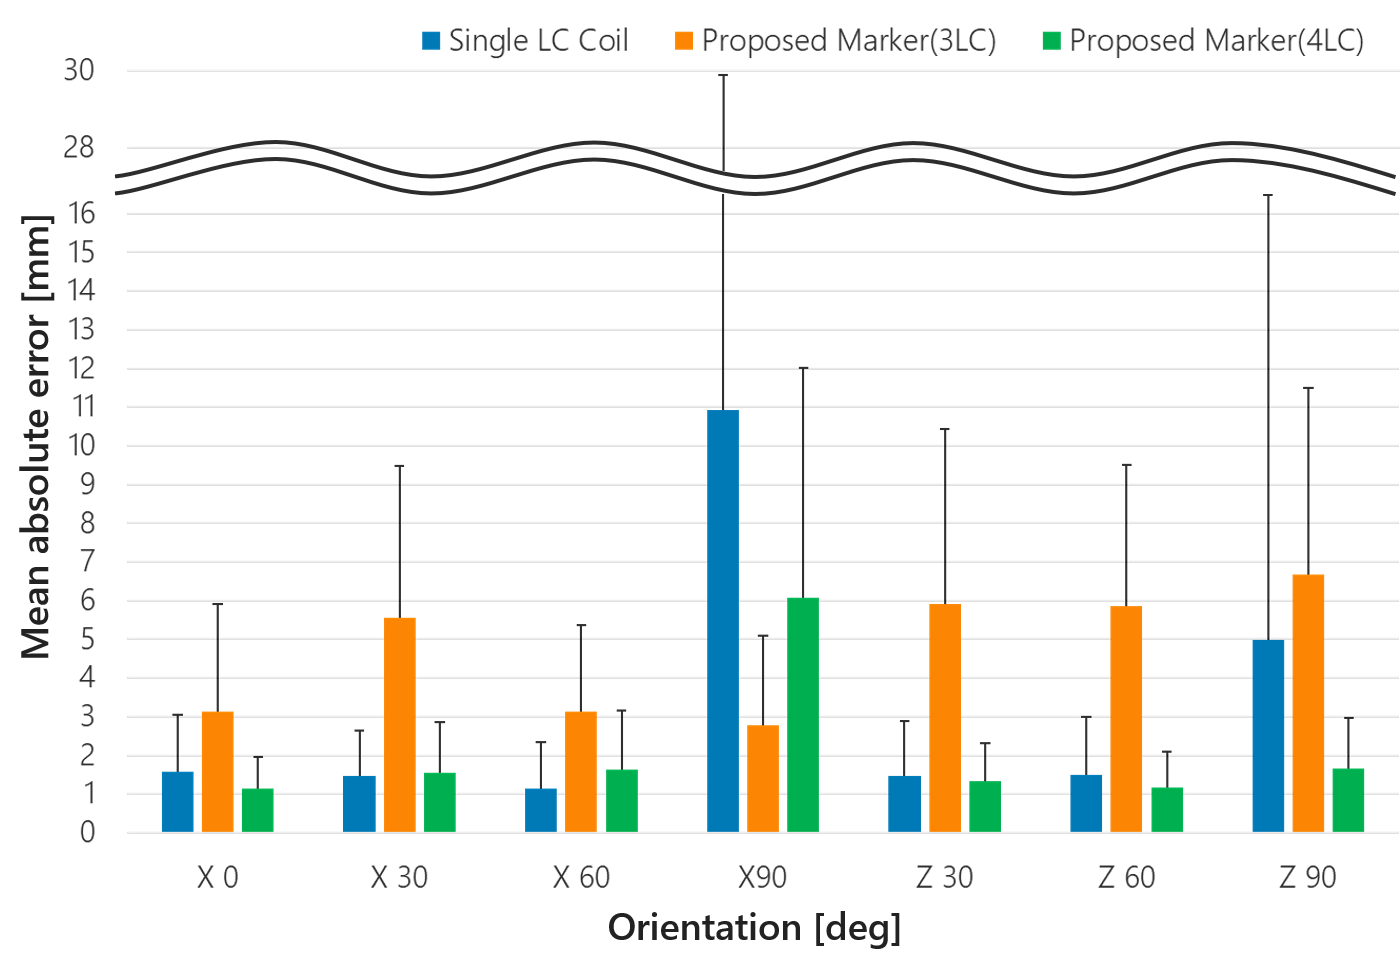
\includegraphics[width=\columnwidth]{figure/yaxis_error2.png}}
    \caption{Mean absolute error of Y axis tracking}
    \label{y-axis-ave_error}
\end{figure}

 \begin{table}[t]
  \begin{center}
  \caption{Y axis tracking errors [mm] (previous work \cite{im3d+})}
  \label{y-axis-error_1LC}
  \begin{tabular}{c||c|c|c} \hline
    Orientation[deg] & MAE & Maximum error & Minimum error\\ \hline\hline
    X 0 & 1.58 & 14.5 & 6.14$\times10^{-4}$ \\
    X 30 & 1.47 & 6.23 & 5.74$\times10^{-3}$ \\
    X 60 & 1.13 & 7.56 & 6.87$\times10^{-4}$ \\
    X 90 & 10.9 & 125 & 1.38$\times10^{-2}$  \\
    Z 30 & 1.47 & 5.86 & 1.17$\times10^{-3}$ \\
    Z 60 & 1.49 & 6.31 & 3.23$\times10^{-4}$ \\
    Z 90 & 4.98 & 127 & 2.40$\times10^{-3}$ \\
  \end{tabular}
  \end{center}
\end{table}

\begin{table}[t]
  \begin{center}
  \caption{Y axis tracking errors [mm] (proposed marker with 3 LC)}
  \label{y-axis-error_3LC}
  \begin{tabular}{c||c|c|c} \hline
    Orientation[deg] & MAE & Maximum error & Minimum error\\ \hline\hline
    X 0 & 3.13 & 16.1 & 4.17$\times10^{-3}$ \\
    X 30 & 5.55 & 20.5 & 1.94$\times10^{-2}$ \\
    X 60 & 3.12 & 19.7 & 5.82$\times10^{-3}$ \\
    X 90 & 2.78 & 19.1 & 7.93$\times10^{-3}$  \\
    Z 30 & 5.90 & 20.2 & 4.56$\times10^{-3}$ \\
    Z 60 & 5.85 & 21.7 & 3.50$\times10^{-3}$ \\
    Z 90 & 6.67 & 27.4 & 1.79$\times10^{-3}$ \\
  \end{tabular}
  \end{center}
\end{table}

\begin{table}[t]
  \begin{center}
  \caption{Y axis tracking errors [mm] (proposed marker with 4 LC)}
  \label{y-axis-error_4LC}
  \begin{tabular}{c||c|c|c} \hline
    Orientation[deg] & MAE & Maximum error & Minimum error\\ \hline\hline
    X 0 & 1.14 & 6.38 & 6.91$\times10^{-4}$ \\
    X 30 & 1.54 & 8.60 & 1.07$\times10^{-3}$ \\
    X 60 & 1.64 & 8.17 & 4.49$\times10^{-3}$ \\
    X 90 & 6.08 & 18.1 & 5.66$\times10^{-3}$  \\
    Z 30 & 1.33 & 5.07 & 1.24$\times10^{-3}$ \\
    Z 60 & 1.16 & 6.95 & 5.65$\times10^{-4}$ \\
    Z 90 & 1.67 & 9.71 & 5.16$\times10^{-4}$ \\
  \end{tabular}
  \end{center}
\end{table}

From the Fig. \ref{y-axis-tracking}, the tracking errors of both the proposed marker and a single LC coil are increasing because the exciting magnetic field strength weakens as the Y-axis coordinates increase. From the Fig. \ref{y-axis-ave_error}, Table \ref{y-axis-error_1LC}, Table \ref{y-axis-error_3LC} and Table \ref{y-axis-error_4LC}, the tracking error of the proposed marker with three LC coils was larger than that of a single LC coil. The proposed marker with four LC coils has the same error as a single LC coil, especially in the dead-angle configuration (X 90$^\circ$ and Z 90$^\circ$), the tracking result of a single LC coil becomes unstable and the error increases. 

In order to measure the error in the horizontal direction, we tracked the pendulum motion on the XZ plane and evaluated the accuracy. The orientation of each marker was the same as in the above experiment. The tracking results is shown in Fig. \ref{pendulum-tracking}. The MAE of tracking is shown in Fig. \ref{pendulum-ave_error}. The error bar shows the standard deviation. In addition, Table \ref{circle-error_1LC}, Table \ref{circle-error_3LC} and Table \ref{pendulum-error_4LC} are show the MAE, maximum and minimum errors of the tracking of a single LC coil and the proposed marker.

\begin{figure*}[t]
  \begin{minipage}{0.5\hsize}
  \begin{center}
   \centerline{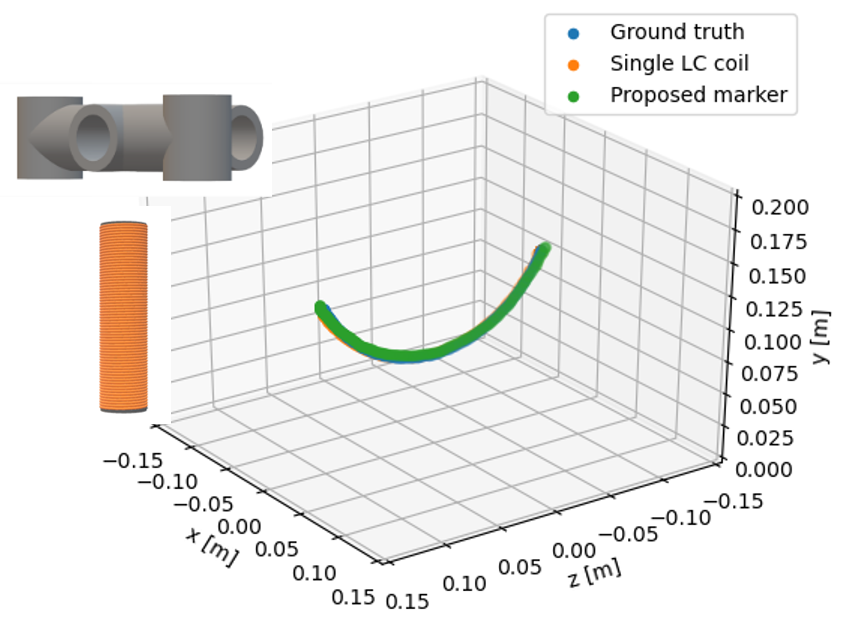
\includegraphics[width=65mm]{figure/pendulum_x-axis_0deg_4LC_2.png}}
  \end{center}
 \end{minipage}
  \begin{minipage}{0.5\hsize}
  \begin{center}
   \centerline{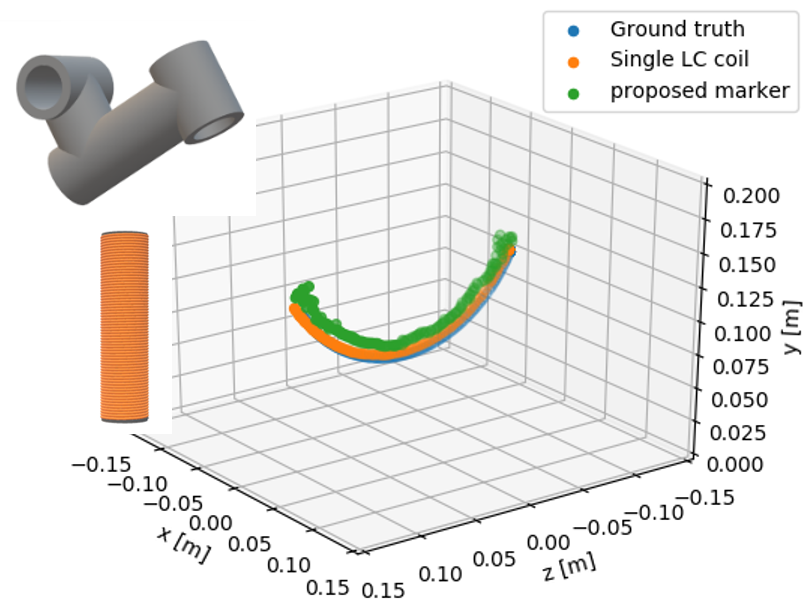
\includegraphics[width=65mm]{figure/pendulum-x0_2.png}}
  \end{center}
 \end{minipage}
 \begin{minipage}{0.5\hsize}
  \begin{center}
   \centerline{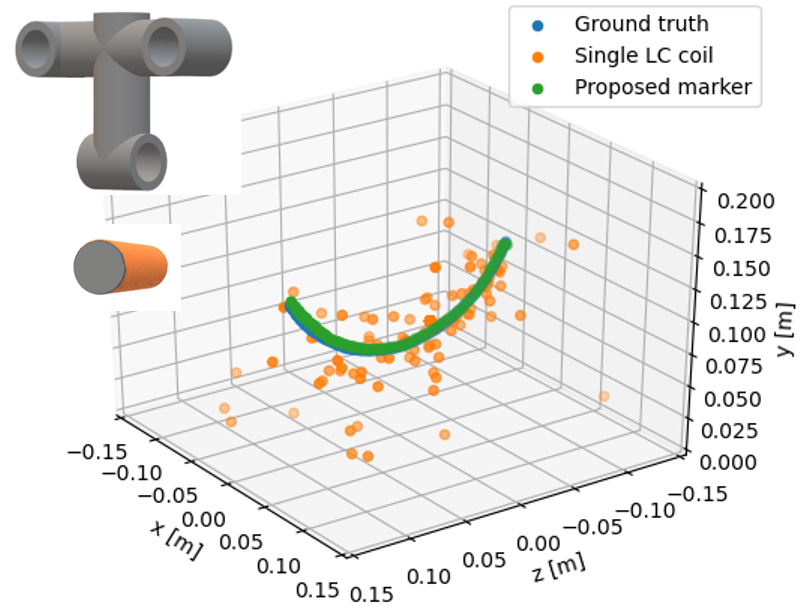
\includegraphics[width=65mm]{figure/pendulum_z-axis_90deg_4LC_2.png}}
  \end{center}
 \end{minipage}
 \begin{minipage}{0.5\hsize}
  \begin{center}
   \centerline{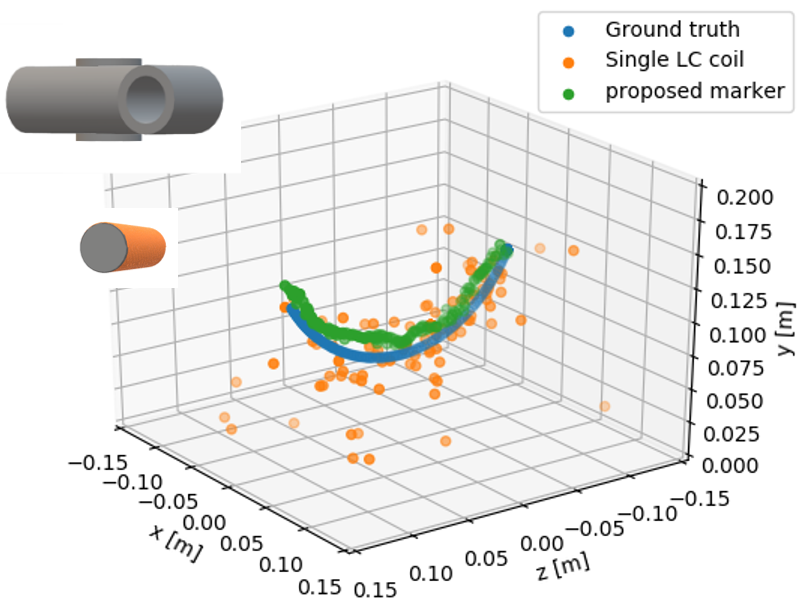
\includegraphics[width=65mm]{figure/pendulum-z90_2.png}}
  \end{center}
 \end{minipage}
 \caption{Pendulum motion tracking results}
 \label{pendulum-tracking}
\end{figure*}
 
 \begin{figure}[!t]
    \centerline{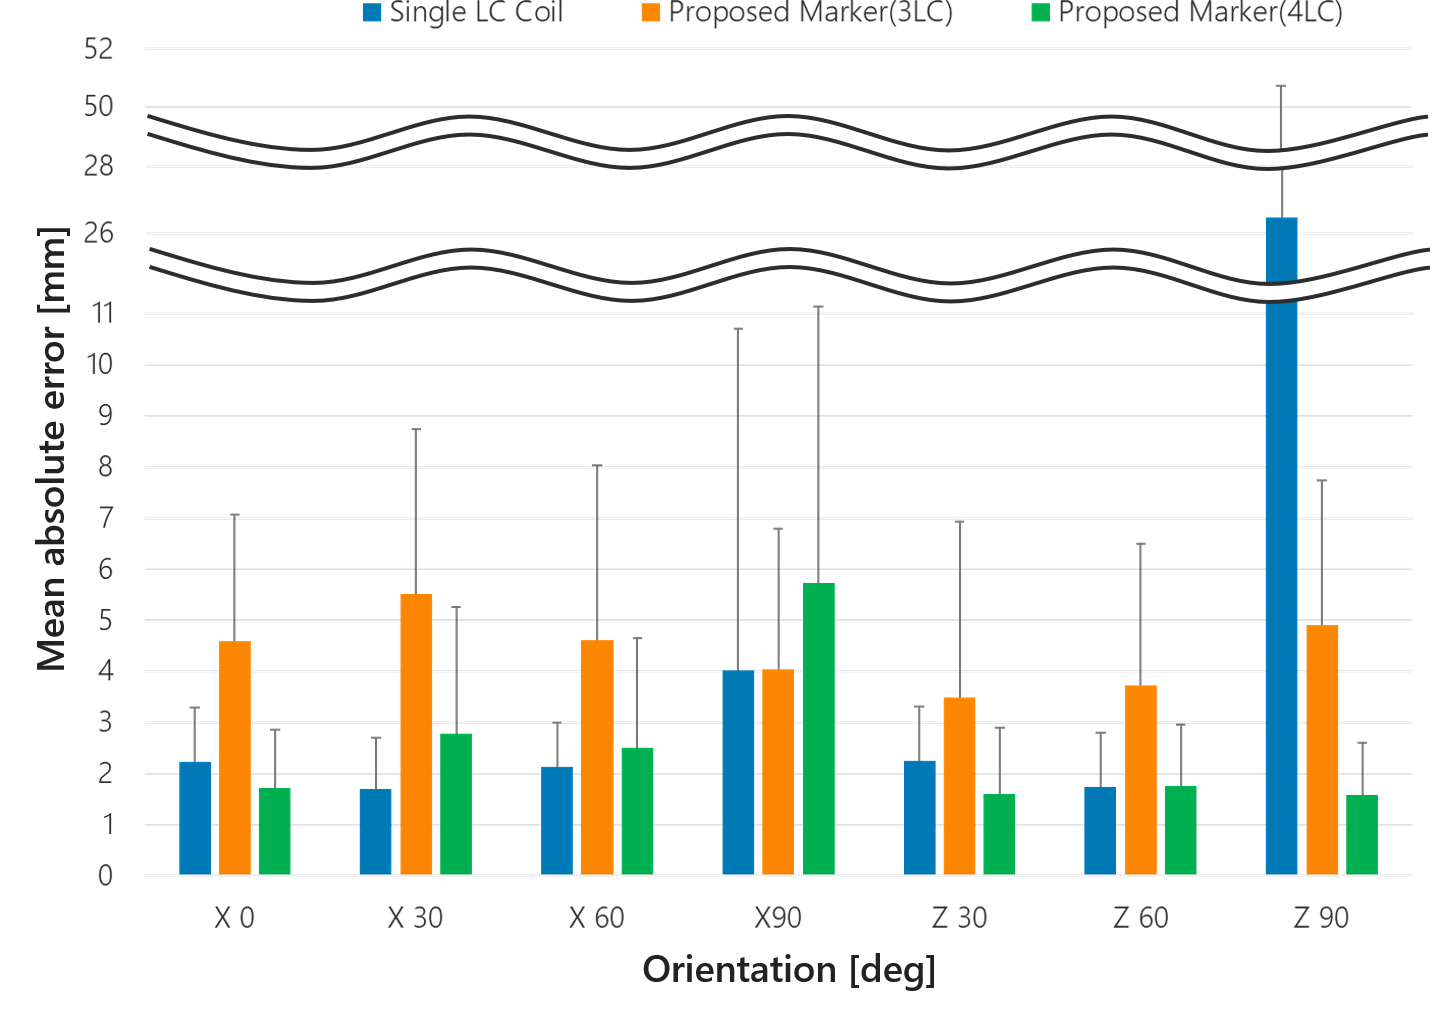
\includegraphics[width=\columnwidth]{figure/pendulum_error2.png}}
    \caption{Mean absolute error of pendulum motion tracking}
    \label{pendulum-ave_error}
\end{figure}

 \begin{table}[t]
  \begin{center}
  \caption{Pendulum motion tracking errors [mm] (previous work \cite{im3d+})}
  \label{pendulum-error_1LC}
  \begin{tabular}{c||c|c|c} \hline
    Orientation[deg] & MAE & Maximum error & Minimum error\\ \hline\hline
    X 0 & 2.23 & 5.13 & 1.72$\times10^{-2}$ \\
    X 30 & 1.70 & 4.04 & 1.06$\times10^{-2}$ \\
    X 60 & 2.14 & 4.54 & 1.26$\times10^{-2}$ \\
    X 90 & 4.03 & 68.9 & 5.93$\times10^{-3}$  \\
    Z 30 & 2.26 & 5.32 & 5.43$\times10^{-3}$ \\
    Z 60 & 1.75 & 4.35 & 7.22$\times10^{-3}$ \\
    Z 90 & 16.5 & 237 & 3.93$\times10^{-2}$ \\
  \end{tabular}
  \end{center}
\end{table}

\begin{table}[t]
  \begin{center}
  \caption{Pendulum motion tracking errors [mm] (proposed marker with 3 LC)}
  \label{pendulum-error_3LC}
  \begin{tabular}{c||c|c|c} \hline
    Orientation[deg] & MAE & Maximum error & Minimum error\\ \hline\hline
    X 0 & 4.59 & 13.8 & 6.29$\times10^{-3}$ \\
    X 30 & 5.52 & 14.6 & 4.54$\times10^{-3}$ \\
    X 60 & 4.60 & 18.1 & 2.49$\times10^{-2}$ \\
    X 90 & 4.04 & 14.2 & 1.37$\times10^{-2}$  \\
    Z 30 & 3.49 & 16.7 & 1.12$\times10^{-2}$ \\
    Z 60 & 3.73 & 14.7 & 1.97$\times10^{-2}$ \\
    Z 90 & 4.91 & 14.5 & 6.37$\times10^{-3}$ \\
  \end{tabular}
  \end{center}
\end{table}

\begin{table}[t]
  \begin{center}
  \caption{Pendulum motion tracking errors [mm] (proposed marker with 4 LC)}
  \label{pendulum-error_4LC}
  \begin{tabular}{c||c|c|c} \hline
    Orientation[deg] & MAE & Maximum error & Minimum error\\ \hline\hline
    X 0 & 1.72 & 4.88 & 2.18$\times10^{-4}$ \\
    X 30 & 2,79 & 11.8 & 1.95$\times10^{-2}$ \\
    X 60 & 2.51 & 10.5 & 1.14$\times10^{-2}$ \\
    X 90 & 5.74 & 15.8 & 5.37$\times10^{-2}$  \\
    Z 30 & 1.60 & 4.91 & 6.41$\times10^{-3}$ \\
    Z 60 & 1.75 & 5.55 & 6.89$\times10^{-3}$ \\
    Z 90 & 1.57 & 4.54 & 4.30$\times10^{-3}$ \\
  \end{tabular}
  \end{center}
\end{table}

From the Fig. \ref{circle-x_4LC} - Fig. \ref{pendulum-z_4LC}, in the configuration of the dead-angle (X 90$^\circ$ and Z 90$^\circ$), the tracking result of a single LC coil becomes unstable in some parts and the error becomes significantly large. From the Fig.\ref{circle-ave_error}, Fig.\ref{pendulum-ave_error} and Table \ref{circle-error_1LC} - Table \ref{pendulum-error_4LC}, proposed marker has the same error as a single LC coil. Especially in the dead-angle configuration (X 90$^\circ$ and Z 90$^\circ$), the tracking result of a single LC coil becomes unstable and the error increases. There is no configuration in which the tracking error of the proposed marker is as large as the dead-angle, but the error tended to increase in a configuration in which only one LC coil in the same marker can be used and all the other LC coils are dead-angle (X 90$^\circ$).

Next, we compared SATBF proposed in \cite{im3d+} with the proposed marker with four LC coils. The problem with SATBF is that the motion cannot be reconstructed correctly if the dead-angle period exceeds the time window size. Therefore, we tracked motions that cause long-term dead angles and evaluated the tracking accuracy of SATBF and the proposed method. The marker is attached to the tip of the robot arm, and a pendulum motion is performed on the XZ plane. The moving speed of the marker was set to 1 [mm/s], and the time window size of the filter was set to 30, which is the same as \cite{im3d+}. When the marker reaches the lowest point of the pendulum, the direction of the marker becomes parallel to the XZ plane, resulting in the dead-angle. The tracking results are shown in the Fig. \ref{filter_result_4LC}.

In the case of a single LC coil, tracking is unstable at the lowest point of the pendulum. Moreover, since the dead-angle period is longer than the time window size of the filter, the motion of the marker cannot be reconstructed correctly even when the motion is reconstructed by applying the filter. On the other hand, the proposed marker has a small error as a whole and can be tracked correctly regardless of the configuration. For this reason, the proposed method is suitable for situations where the configuration of the marker is close to the dead-angle in the long term.

\begin{figure}[t]
    \centering
    \centerline{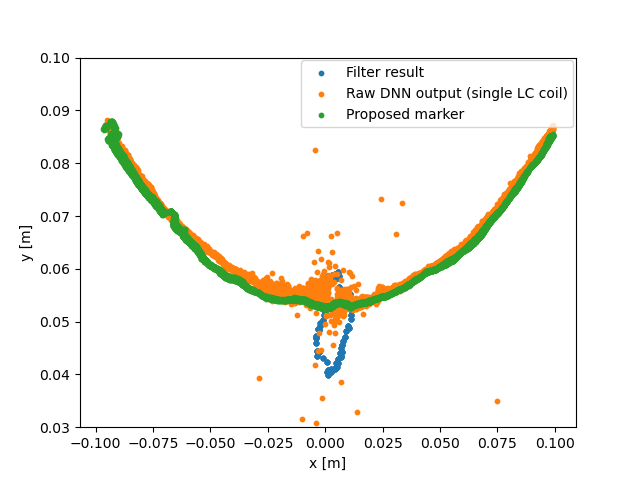
\includegraphics[width=\columnwidth]{figure/filter_result_4LC.png}}
    \caption{Comparison of SATBF and proposed marker with four LC coils}
    \label{filter_result_4LC}
\end{figure}

\subsection{Processing speed}
In \cite{im6d}, the Gauss-Newton method was used for marker tracking, but in this work, we adopted DNN, which can be expected to perform high-speed calculation without considering the initial value. Therefore we compared the relationship between the calculation performance of marker tracking and the number of markers that can be used simultaneously on the system bitween \cite{im6d} and proposed method. The results are shown in Fig. \ref{speed}.

The processing speed of \cite{im6d} decreases significantly as the number of markers that can be used simultaneously increases. On the other hand, the proposed method has a stable processing speed even when the number of markers that can be used simultaneously increases. However, the processing speed of the DNN method is limited by the sampling frequency of the A/D converters. For this reason, the DNN approach is robust because it does not require consideration of initial values, and is superior to the Gauss-Newton method in terms of processing speed. Moreover, in \cite{im6d}, by using three LC coils with different resonance frequencies for the markers, the number of markers that can be used simultaneously on the system is reduced to 1/3, but the proposed method can use markers up to the maximum number in the hardware specifications.

\begin{figure}[t]
    \centerline{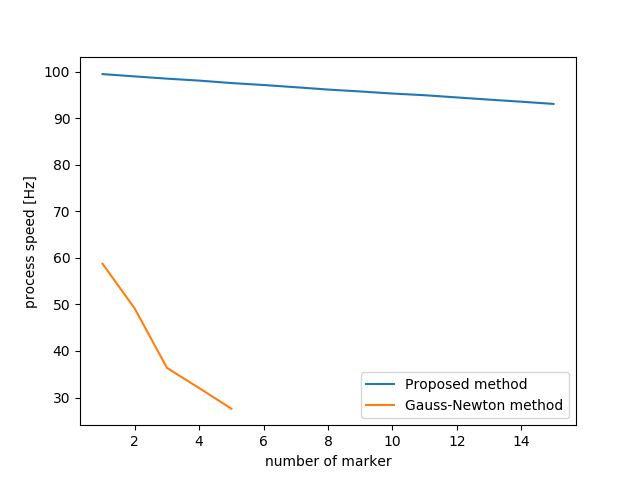
\includegraphics[width=\columnwidth]{figure/speed.png}}
    \caption{Processing speed of DNN and Gauss-Newton method}
    \label{speed}
\end{figure}

\section{Application example}
An important contribution of the proposed method is that tracking can be continued stably even if the dead-angle is long-term without depending on the configuration of the marker. In addition, the number of markers that can be used simultaneously, which was a problem in \cite{im6d}, was solved at the same time. As a situation where the dead-angle actually occurs for a long time, We attached the markers to objects such as blocks that easily keeps a certain configuration, and created an application that becomes the dead-angle when the blocks fall down (Fig. \ref{domino}). When blocks fall down, the tracking of some blocks becomes unstable in the case of a single LC coil because the dead-angle configuration is maintained for a long time, however the proposed marker can continue tracking without depending on the posture.

In order to demonstrate whether the proposed method can perform as well as the previous work \cite{im3d, im6d, im3d+}, we evaluated the system in the actual possible application situations.

For tracking finger motion and finger-object interaction, small, lightweight, wireless, occlusion-free markers is required so as not to interfere with finger movement. Since the proposed marker is small, lightweight, and wireless, it can be attached to the fingertip to track the natural interaction between the objects and the fingers (Fig. \ref{mug}). In addition, because our system is magnetic, tracking can be continued even if occlusion occurs.

Since the proposed marker is small, it can be attached to various objects as well as fingertips for tracking. You can put a marker inside the capsule as shown in the Fig. \ref{capsule_cloth} to continue tracking even if the object is hidden in the bag and occlusion occurs.
By placing a marker inside a sealed object such as a capsule and tracking it, it is possible to track the natural movement of an object underwater. In the optical motion tracking system, it is difficult to track the marker due to the complex light reflection of water, and in the case of an opaque liquid, tracking becomes impossible due to occlusion, but our method is magnetic and can continue tracking.
\begin{figure}[t]
    \centerline{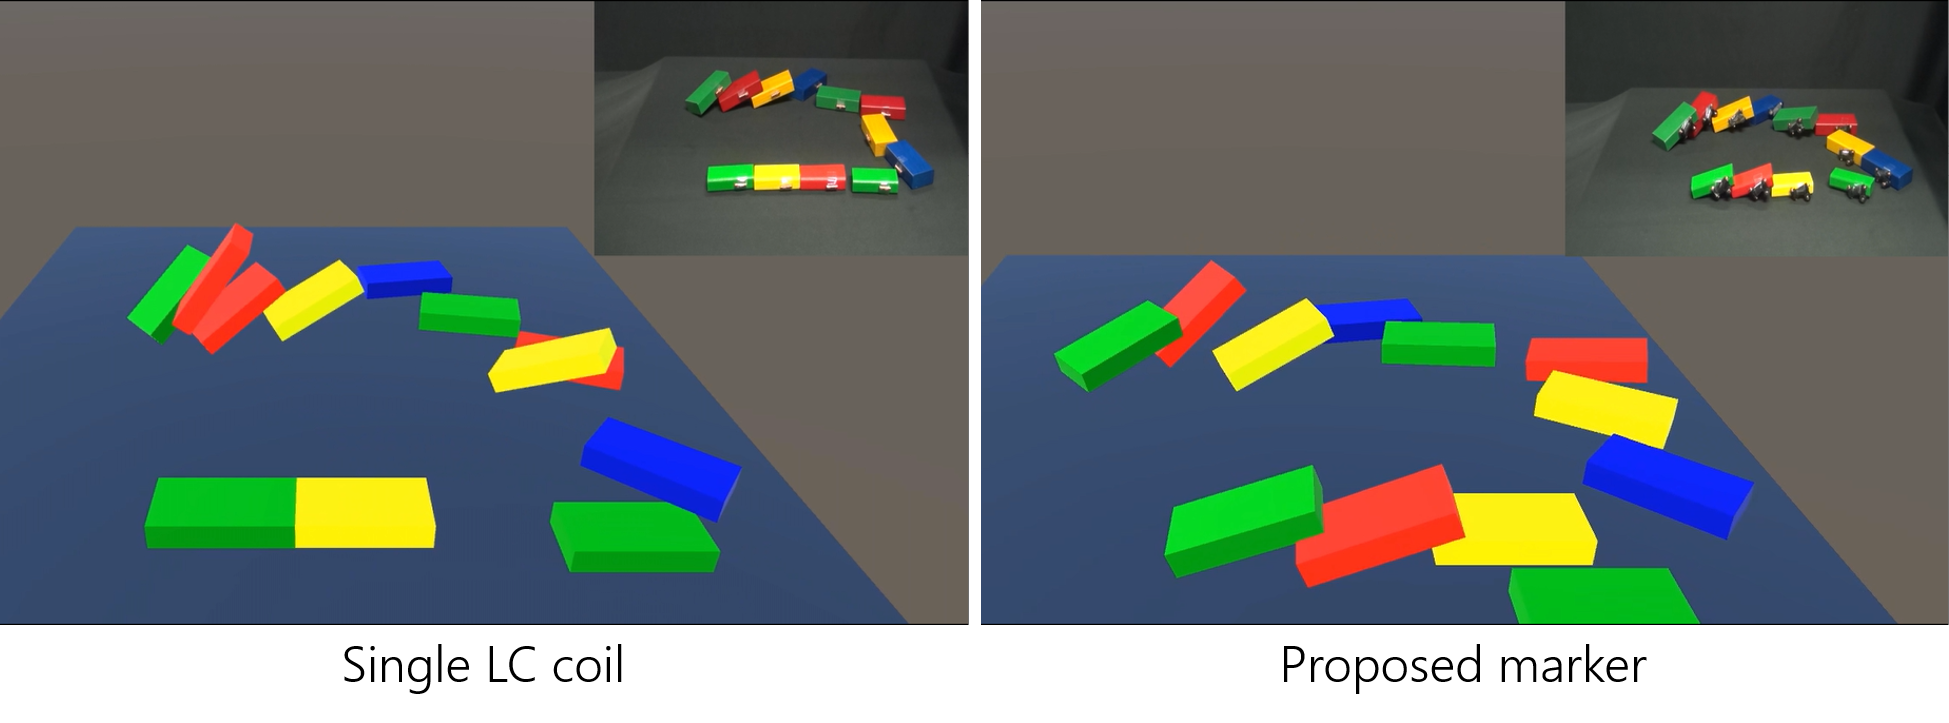
\includegraphics[width=\columnwidth]{figure/domino.png}}
    \caption{Situations where dead angles occur in the long term}
    \label{domino}
\end{figure}
\begin{figure}[t]
    \centerline{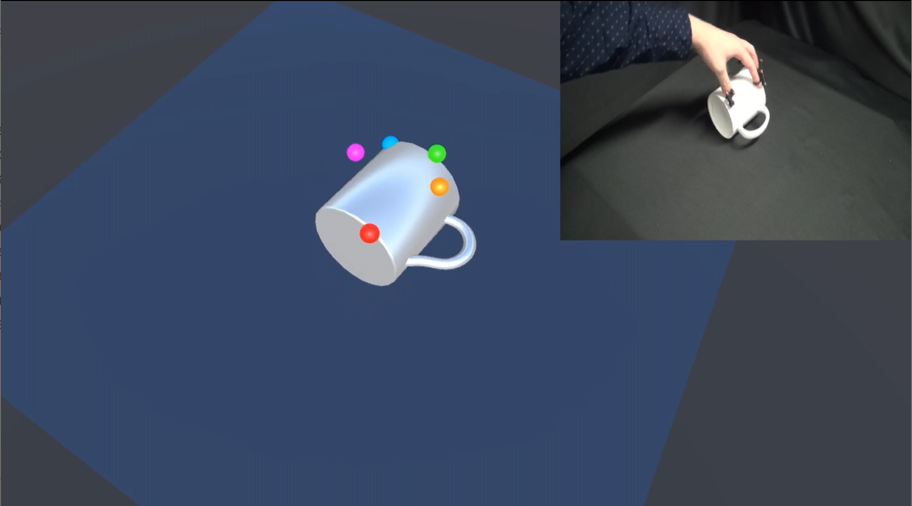
\includegraphics[width=\columnwidth]{figure/mug.png}}
    \caption{Hand-object interaction}
    \label{mug}
\end{figure}
\begin{figure}[t]
    \centerline{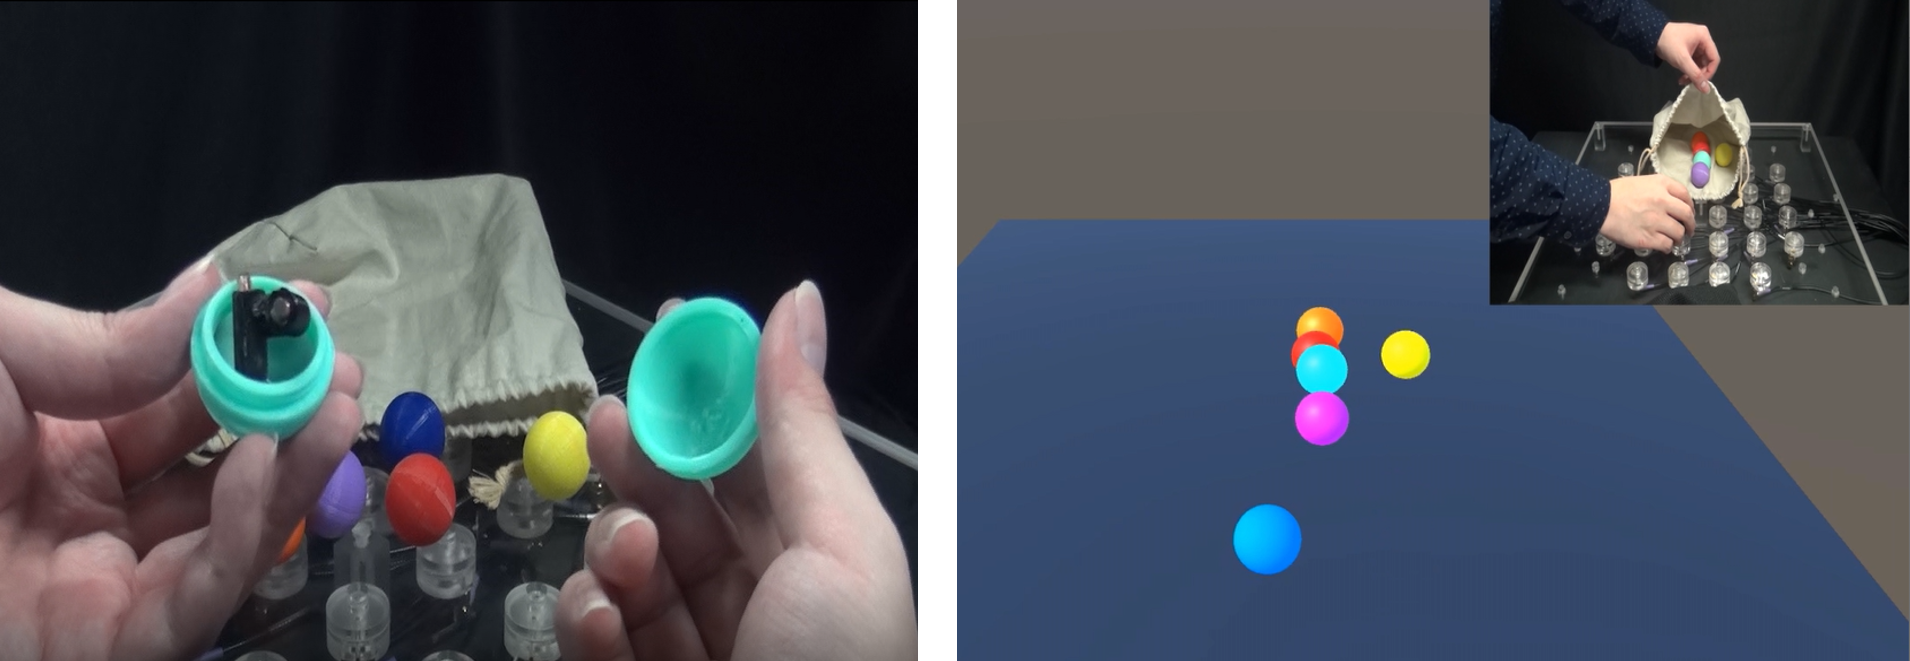
\includegraphics[width=\columnwidth]{figure/capsule_cloth.png}}
    \caption{Tracking objects in a bag}
    \label{capsule_cloth}
\end{figure}
\begin{figure}[t]
    \centerline{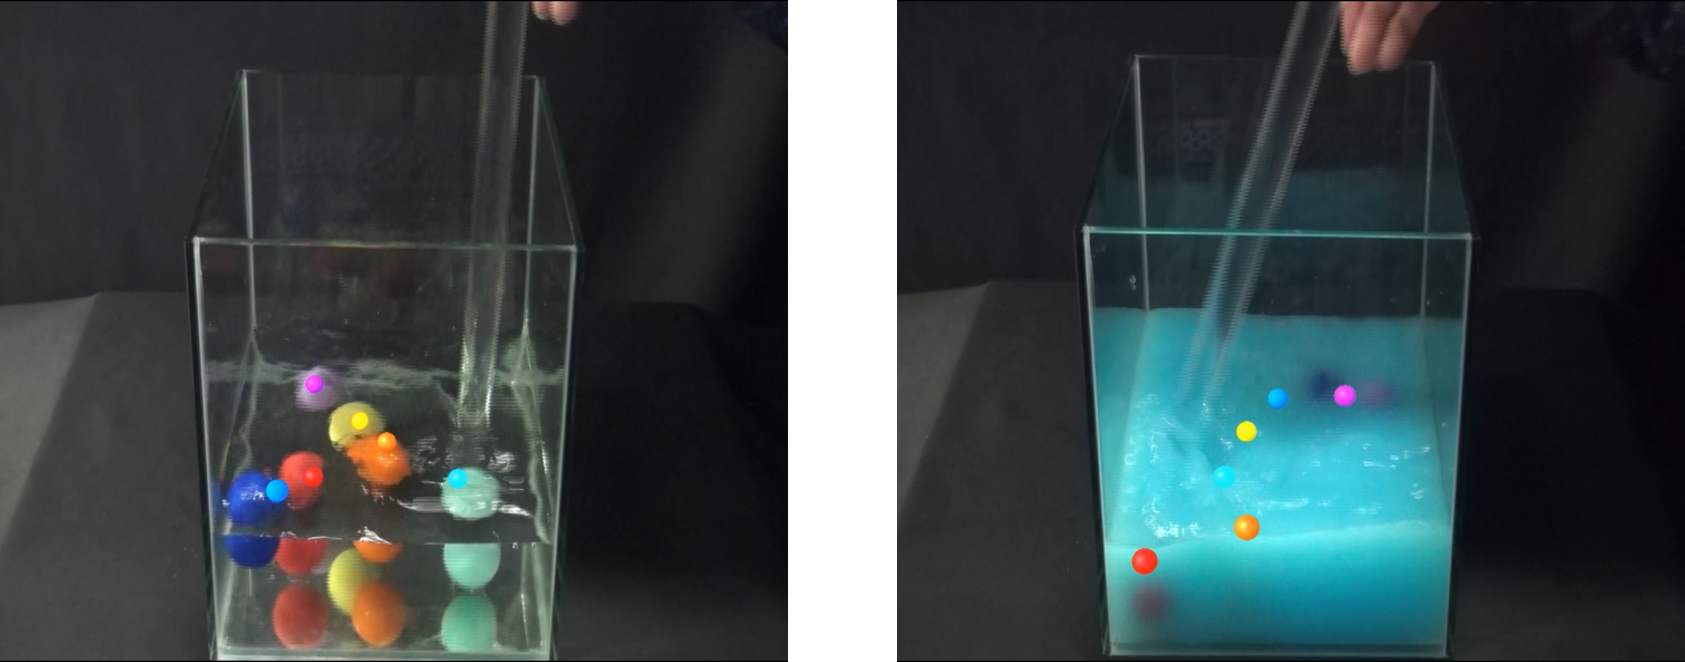
\includegraphics[width=\columnwidth]{figure/capsule_water.png}}
    \caption{Tracking objects in water}
    \label{capsule_water}
\end{figure}

\section{Discussion}
The results show that the tracking accuracy of the proposed marker with three LC coils was inferior to that of a single LC coil except for the dead-angle. The tracking accuracy of the proposed marker with four LC coils was significantly improved compared to the marker with three LC coils by increasing the number of LC coils in the same marker, but the error tended to be larger in some configurations. The most important factor for this is the ambiguity of DNN mapping. In the proposed marker design, each LC coil is arranged orthogonally to reduce the influence of cross-coupling, however there are configurations in which only one LC coil within the same marker is available and all other LC coils are the dead-angle. In such configurations, the positions of the marker of multiple patterns are mapped to the distribution of the flux sensors' output of one pattern, and it is considered that the error is large.

The second factor is the individual difference of the LC coil set with the same resonance frequency characteristics. In the proposed DNN, the induced strengths of the LC coils that make up the marker are assumed to be equal, however in reality there are individual differences in each LC coil. In the experiment, FFT analysis is performed by selecting frequencies that reduce the influence of individual differences, however it is difficult to completely equalize the induced strengths of the LC coils.

The third factor is the error in frequency characteristics due to interference between LC coils. The proposed marker was designed so that the effect of cross-coupling due to interference between LC coils was reduced, however the effect of interference was not completely eliminated. Therefore, it is considered that there is an error between the measured value obtained by FFT analysis of the measured value of the flux sensors and the theoretical value calculated theoretically.

As a method for improving the performance of the system, a marker design in which the number of LC coils in the same marker is increased can be considered. Increasing the number of LC coils can reduce the DNN mapping error, which is thought to lead to improved accuracy. Another possible method is to use a set of LC coils with accurate resonance frequency characteristics. By aligning the resonance frequency characteristics, the contribution of each LC coil in FFT analysis can be accurately measured, and the resonance magnetic flux of the marker can be theoretically calculated.

\section{Conclusion}
In this work, in order to solve the problems of the magnetic motion tracking system, which is the previous work, the long-term dead-angle and the decrease in the number of markers that can be used simultaneously, we proposed the marker with multiple LC coils with the same resonance frequency. We showed that the DNN solver can successfully solve the analysis of complex electromagnetically related signal sources, which is difficult with numerical models.

As a result of the performance evaluation, we confirmed that the dead-angle could be solved by using the proposed marker, and the tracking accuracy was significantly improved for the marker with four LC coils than for the marker with three LC coils. It was possible to solve the long-term dead-angle and the decrease in the number of markers that can be used simultaneously, and it was shown that it could be applied to tasks that were difficult with existing systems.

The error tends to increase with respect to some configurations of the proposed marker, and the reason may be the ambiguity of DNN mapping due to the characteristics of the marker design. In addition, the factors of the overall error are considered to be the individual differences in the resonance frequency characteristics of the LC coil and the influence of interference between the LC coils. Possible improvements include studying a marker design that has characteristics that enable accurate mapping with DNN, such as increasing the number of LC coils in the same marker, and manufacturing LC coils that have accurate resonance frequency characteristics. Through these works, it may be possible to improve the performance of the method proposed.

\begin{thebibliography}{00}

\bibitem{polhemus} ``Polhemus,'' \url{http://polhemus.com/}. (2020/11/20).

\bibitem{tensorflow} ``TensorFlow,'' \url{https://www.tensorflow.org/}. (2020/11/20).

\bibitem{keras} ``Keras,'' \url{https://keras.io/}. (2020/11/20).

\bibitem{im3d} Jiawei Huang, Kazuki Takashima, Shuichiro Hashi, and Yoshifumi Kitamura, ``IM3D: Magnetic motion tracking system for dexterous 3D interactions,'' \emph{In ACM SIGGRAPH 2014 Emerging Technologies}, 2014.

\bibitem{im6d} Jiawei Huang, Tsuyoshi Mori, Kazuki Takashima, Shuichiro Hashi,
and Yoshifumi Kitamura, `` IM6D: Magnetic tracking system with 6-
DOF passive markers for dexterous 3D interaction and motion,'' \emph{ACM Transactions on Graphics}, Vol. 34, No. 6, 2015.

\bibitem{yabukami1} Shin Yabukami, Shuichiro Hashi, Yuki Tokunaga, Takeshi Kohno,
Ken Ichi Arai, and Yasuo Okazaki, ``Development of a positionsensing system for a wireless magnetic marker,'' \emph{Journal of the Magnetics Society of Japan}, Vol. 28, No. 7, pp. 877–885, 2004.

\bibitem{hashi1} Shuichiro Hashi, Masaharu Toyoda, Shin Yabukami, Kazushi
Ishiyama, Yasuo Okazaki, Ken Ichi Arai, and Hiroyasu Kanetaka, ``DWireless magnetic motion capture system using multiple LC resonant magnetic markers with high accuracy,'' \emph{Sensors and Actuators A: Physical}, Vol. 142, No. 2, pp. 520–527, 2008.

\bibitem{im3d+} Jiawei Huang, Ryo Sugawara, Kinfung Chu, Taku Komura, and
Yoshifumi Kitamura, ``Reconstruction of dexterous 3D motion data
from a flexible magnetic sensor with deep learning and structureaware filtering,'' \emph{IEEE Transactions on Visualization and Computer Graphics}, 2020, Early Access.

\bibitem{gaussbits} Rong-Hao Liang, Kai-Yin Cheng, Liwei Chan, Chuan-Xhyuan Peng,
Mike Y. Chen, Rung-Huei Liang, De-Nian Yang, and Bing-Yu Chen, ``GaussBits: Magnetic tangible bits for portable and occlusion-free
near-surface interactions,'' \emph{In Proceedings of the SIGCHI Conference
on Human Factors in Computing Systems}, p. 1391–1400, 2013.

\bibitem{gaussrfid} Rong-Hao Liang, Han-Chih Kuo, and Bing-Yu Chen, ``GaussRFID:
Reinventing physical toys using magnetic RFID development kits,'' \emph{In Proceedings of the 2016 CHI Conference on Human Factors in
Computing Systems},  p. 4233–4237, 2016.

\bibitem{utrack} Ke-Yu Chen, Kent Lyons, Sean White, and Shwetak Patel, `` uTrack:
3D input using two magnetic sensors,'' \emph{In Proceedings of the 26th
annual ACM symposium on User interface software and technology},  p. 237–244, 2013.

\bibitem{fem} A. Fernandez G. David, Enrico Macrelli, Danilo Demarchi, and
Marco Crepaldi, ``High-accuracy wireless 6DOF magnetic tracking
system based on FEM modeling,'' \emph{ In 25th IEEE International Conference on Electronics, Circuits and Systems},  pp. 413–416, 2018.

\bibitem{magne_inert} Houde Dai, Shuang Song, Chao Hu, Bo Sun, and Zhirong Lin, ``A
novel 6D tracking method by fusion of 5D magnetic tracking and
3D inertial sensing,'' \emph{IEEE Sensors Journal},   pp. 9640–9648, 2018.

\bibitem{intr_cap_magne_sens} Peter Sandilands, Myung Geol Choi, and Taku Komura, ``Interaction capture using magnetic sensors,'' \emph{Computer Animation and
Virtual Worlds},  Vol. 24, No. 6, pp. 527–538, 2013.

\bibitem{finexus} Ke-Yu Chen, Shwetak N. Patel, and Sean Keller, ``Finexus: Tracking precise motions of multiple fingertips using magnetic sensing,'' \emph{In Proceedings of the 2016 CHI Conference on Human Factors in
Computing Systems}, p. 1504–1514, 2016.

\bibitem{auraring} Farshid Salemi Parizi, Eric Whitmire, and Shwetak Patel, ``AuraRing: Precise electromagnetic finger tracking,'' \emph{Proceedings of the
ACM on Interactive, Mobile, Wearable and Ubiquitous Technologies}, Vol. 3, No. 4, 2019.

\bibitem{paperio} Zhu Kening, Rongbo Zhu, Hideaki Nii, Hooman Samani, and
Borhan Jalaeian, `` PaperIO: A 3D interface towards the internet
of embedded paper-craft,'' \emph{IEICE Transactions on Information and
Systems}, Vol. 97, pp. 2597–2605, 10 2014.

\bibitem{four_ext_coil} Yutaro Osaki, Shuichiro Hashi, Shin Yabukami, Kanetaka Hiroyasu, and Kazushi Ishiyama, ``Wireless magnetic position-detection
system with four excitation coils,'' \emph{IEEE Sensors Journal}, Vol. 17,
No. 14, pp. 4412–4419, 2017.

\bibitem{cross-coupling} Takehiro Imura, ``Equivalent circuits of repeater antennas for wireless power transfer via magnetic resonant coupling,'' \emph{IEEJ Transactions on Industry Applications}, Vol. 131, pp. 1373–1382, 2011.

\bibitem{cross-coupling2} Gunbok Lee, Benjamin Waters, Brody Mahoney, Joshua Smith,
and Wee Park, ``An investigation of cross-coupling for magnetically
coupled wireless power transfer,'' \emph{ In 2013 Asia-Pacific Microwave
Conference Proceedings},  pp. 80–82, 2013.

\bibitem{squarecoil} Martin Misakian, ``Equations for the magnetic field produced by
one or more rectangular loops of wire in the same plane,'' \emph{Journal
of Research of the National Institute of Standards and Technology},  Vol. 105, pp. 557–564, 2000.

\bibitem{adam} Diederik Kingma and Jimmy Ba, ``Adam: A method for stochastic
optimization,'' \emph{ In International Conference on Learning Representations}, 2015.

\end{thebibliography}

\begin{IEEEbiography}[{\includegraphics[width=1in,height=1.25in,clip,keepaspectratio]{a1.png}}]{First A. Author} (M'76--SM'81--F'87) and all authors may include 
biographies. Biographies are often not included in conference-related
papers. This author became a Member (M) of IEEE in 1976, a Senior
Member (SM) in 1981, and a Fellow (F) in 1987. The first paragraph may
contain a place and/or date of birth (list place, then date). Next,
the author's educational background is listed. The degrees should be
listed with type of degree in what field, which institution, city,
state, and country, and year the degree was earned. The author's major
field of study should be lower-cased. 

The second paragraph uses the pronoun of the person (he or she) and not the 
author's last name. It lists military and work experience, including summer 
and fellowship jobs. Job titles are capitalized. The current job must have a 
location; previous positions may be listed 
without one. Information concerning previous publications may be included. 
Try not to list more than three books or published articles. The format for 
listing publishers of a book within the biography is: title of book 
(publisher name, year) similar to a reference. Current and previous research 
interests end the paragraph. The third paragraph begins with the author's 
title and last name (e.g., Dr.\ Smith, Prof.\ Jones, Mr.\ Kajor, Ms.\ Hunter). 
List any memberships in professional societies other than the IEEE. Finally, 
list any awards and work for IEEE committees and publications. If a 
photograph is provided, it should be of good quality, and 
professional-looking. Following are two examples of an author's biography.
\end{IEEEbiography}

\begin{IEEEbiography}[{\includegraphics[width=1in,height=1.25in,clip,keepaspectratio]{a2.png}}]{Second B. Author} was born in Greenwich Village, New York, NY, USA in 
1977. He received the B.S. and M.S. degrees in aerospace engineering from 
the University of Virginia, Charlottesville, in 2001 and the Ph.D. degree in 
mechanical engineering from Drexel University, Philadelphia, PA, in 2008.

From 2001 to 2004, he was a Research Assistant with the Princeton Plasma 
Physics Laboratory. Since 2009, he has been an Assistant Professor with the 
Mechanical Engineering Department, Texas A{\&}M University, College Station. 
He is the author of three books, more than 150 articles, and more than 70 
inventions. His research interests include high-pressure and high-density 
nonthermal plasma discharge processes and applications, microscale plasma 
discharges, discharges in liquids, spectroscopic diagnostics, plasma 
propulsion, and innovation plasma applications. He is an Associate Editor of 
the journal \emph{Earth, Moon, Planets}, and holds two patents. 

Dr. Author was a recipient of the International Association of Geomagnetism 
and Aeronomy Young Scientist Award for Excellence in 2008, and the IEEE 
Electromagnetic Compatibility Society Best Symposium Paper Award in 2011. 
\end{IEEEbiography}

\begin{IEEEbiography}[{\includegraphics[width=1in,height=1.25in,clip,keepaspectratio]{a3.png}}]{Third C. Author, Jr.} (M'87) received the B.S. degree in mechanical 
engineering from National Chung Cheng University, Chiayi, Taiwan, in 2004 
and the M.S. degree in mechanical engineering from National Tsing Hua 
University, Hsinchu, Taiwan, in 2006. He is currently pursuing the Ph.D. 
degree in mechanical engineering at Texas A{\&}M University, College 
Station, TX, USA.

From 2008 to 2009, he was a Research Assistant with the Institute of 
Physics, Academia Sinica, Tapei, Taiwan. His research interest includes the 
development of surface processing and biological/medical treatment 
techniques using nonthermal atmospheric pressure plasmas, fundamental study 
of plasma sources, and fabrication of micro- or nanostructured surfaces. 

Mr. Author's awards and honors include the Frew Fellowship (Australian 
Academy of Science), the I. I. Rabi Prize (APS), the European Frequency and 
Time Forum Award, the Carl Zeiss Research Award, the William F. Meggers 
Award and the Adolph Lomb Medal (OSA).
\end{IEEEbiography}

\end{document}
